\section{Growth of non-axisymmetric modes without the influence of the
  planet}\label{linear1}
In this section, the planet is introduced at $t=20P_0$ and 
its potential switched on over $10P_0$. At $t=30P_0$ we switch off the
planet potential and azimuthally average the surface density, energy
and velocity fields. At this point the planet has carved a partial
gap and the RWI has not yet occured.
 We then perturb the surface density for $r>r_p$ and continue to 
evolve the disc. We impose  sinusoidal perturbations with 
azimuthal wavenumbers $m\in[1,10]$ and random amplitudes within $\pm 0.01$
 times the local surface density.% {\bf what are PERTMIN and PERTMAX values?}  
This procedure allows us to analyse the growth of 
non-axisymmetric modes associated with the gap, but without
complications from non-axisymmetry arising directly from disc-planet
interaction.

Note that these `planet-off' simulations are not linear stability
calculations because since the cooling term in our energy equation
restores the initial temperature profile corresponding to $H/r=0.05$,
rather than the heated gap edge. Linear stability calculations and
adiabatic cases will be further discussed in
section~\ref{adiabatic_section}.  


Simulations here employ a resolution of $(N_r,N_{\phi})=(1024,2048)$
with an open boundry condition at the outer disk edge $r_\mathrm{out}=25r_\mathrm{in}$. We consider 
%for a time up to $200P_0$ allowing high resolution and detection of high
%$m$ structures.
cases of $\tilde{\beta}=0.1,1,10$ corresponding to fast, moderate,
and slowly cooled discs. % {\bf boundary condition for these sims?}

\subsection{Gap structure}
%Since stability of the gap is of interest 
We first examine the gap structure formed by planet-disc
interaction as a function of the cooling time. The azimuthally-averaged 
gap profiles are shown in Fig. \ref{intial1D} for varying
$\tilde\beta$. Gaps formed with lower $\tilde\beta$ (faster cooling)
are deeper with steeper gradients at the gap edges. Faster cooling rates also 
increase and decrease the surface density maxima and 
minima increase, respectively. However, a clean gap does not form
in this short time period. 

%For all cases the gap width is $\approx 5r_{hill}$
%which is set by torque balances in the disk \citep{crida06}. 

Larger $\tilde\beta$ values result in higher disc aspect ratios $h=H/r$,
i.e. higher temperatures. Heating mostly occur at the gap edges
due to planet-induced spiral shocks. Decreasing the cooling time
implies that this heat is retained in the disc. In the inviscid limit the gap
opening condition is $r_h\gtrsim H$ or $q\gtrsim 3h^3$
\citep{crida06}. 
% which is a value directly correlated to temperature in our model. 
%For a planet to carve a gap in the surrounding material it has been
%shown that $q>H^3$ is needed \citep{crida06}. 
This indicates that for hotter discs (higher
$h$), it becomes more difficult for a planet of fixed $q$ to open a
gap. This explains the shallower gaps in surface density when
$\tilde{\beta}$ is increased. 

%This is seen in our simulations as changes in $\tilde{\beta}$
%result in changes of $h$ by less than $20\%$ yet gap depth almost
%doubles. 

The important consequence of a heated gap edge is that the
generalized vortensity profiles become smoother with increasing
cooling times, with the extrema becoming less pronounced. Previous locally
isothermal disc-planet simulations show the RWI associated with PV
minima \citep{li05,lin10}. We can therefore expect the RWI to be associated with
minima in the generalized vortensity (corresponding to local surface
density maxima) in the non-isothermal case. Because the extrema are
less sharp, the RWI is expected to be weaker and the gap to be more
stable with longer cooling times.  

%Charactereristicly
%for such disk-planet Rossby vortices the generalized vortensity
%minima correspond to density maxima in the disk. 
%Since generalized vortensity extrema are also
% correspondingly less pronounced and density gradients become smaller
% we expect that the stability of gaps to increase with larger
% $\tilde{\beta}$. 

\begin{figure}
  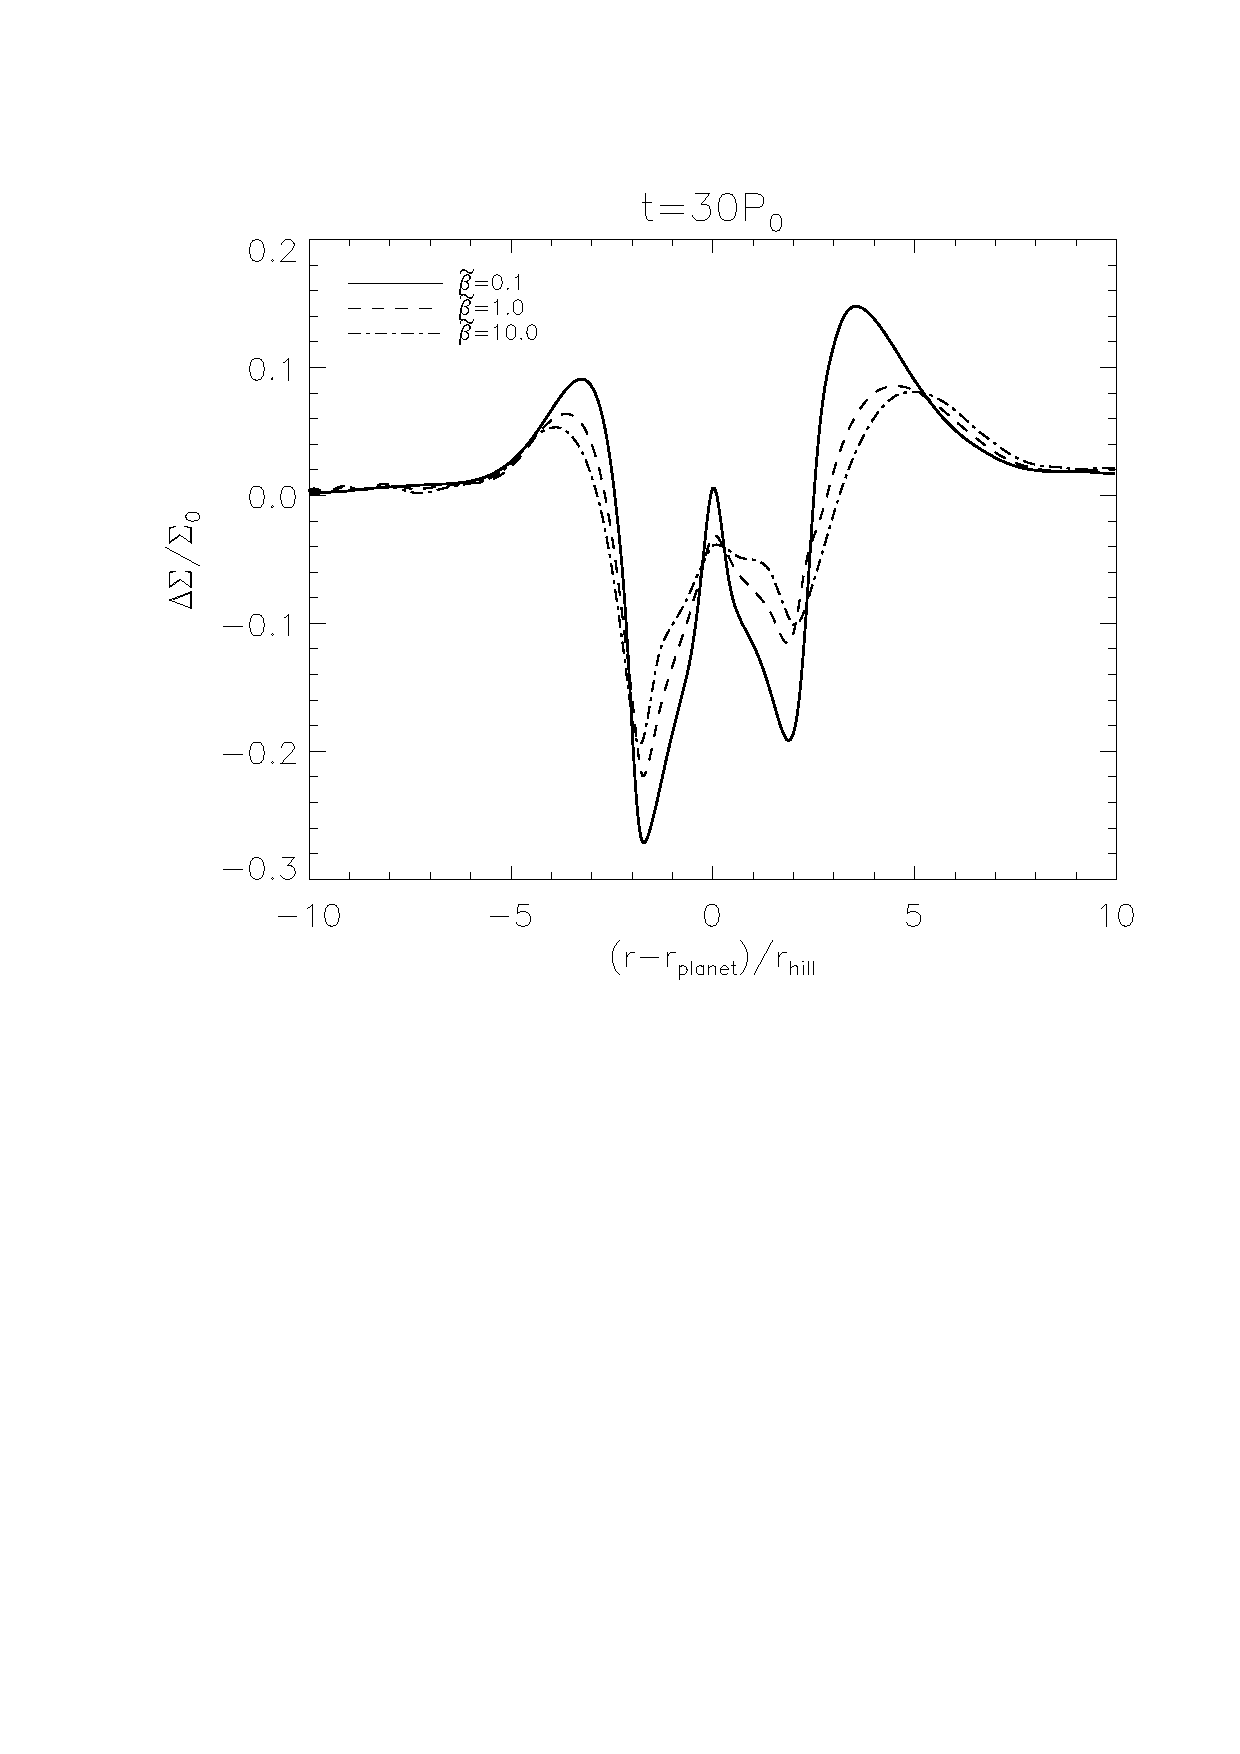
\includegraphics[width=\linewidth,clip=true,trim=0.5cm
    2cm 0cm 0cm]{figures/compare_sigma}
  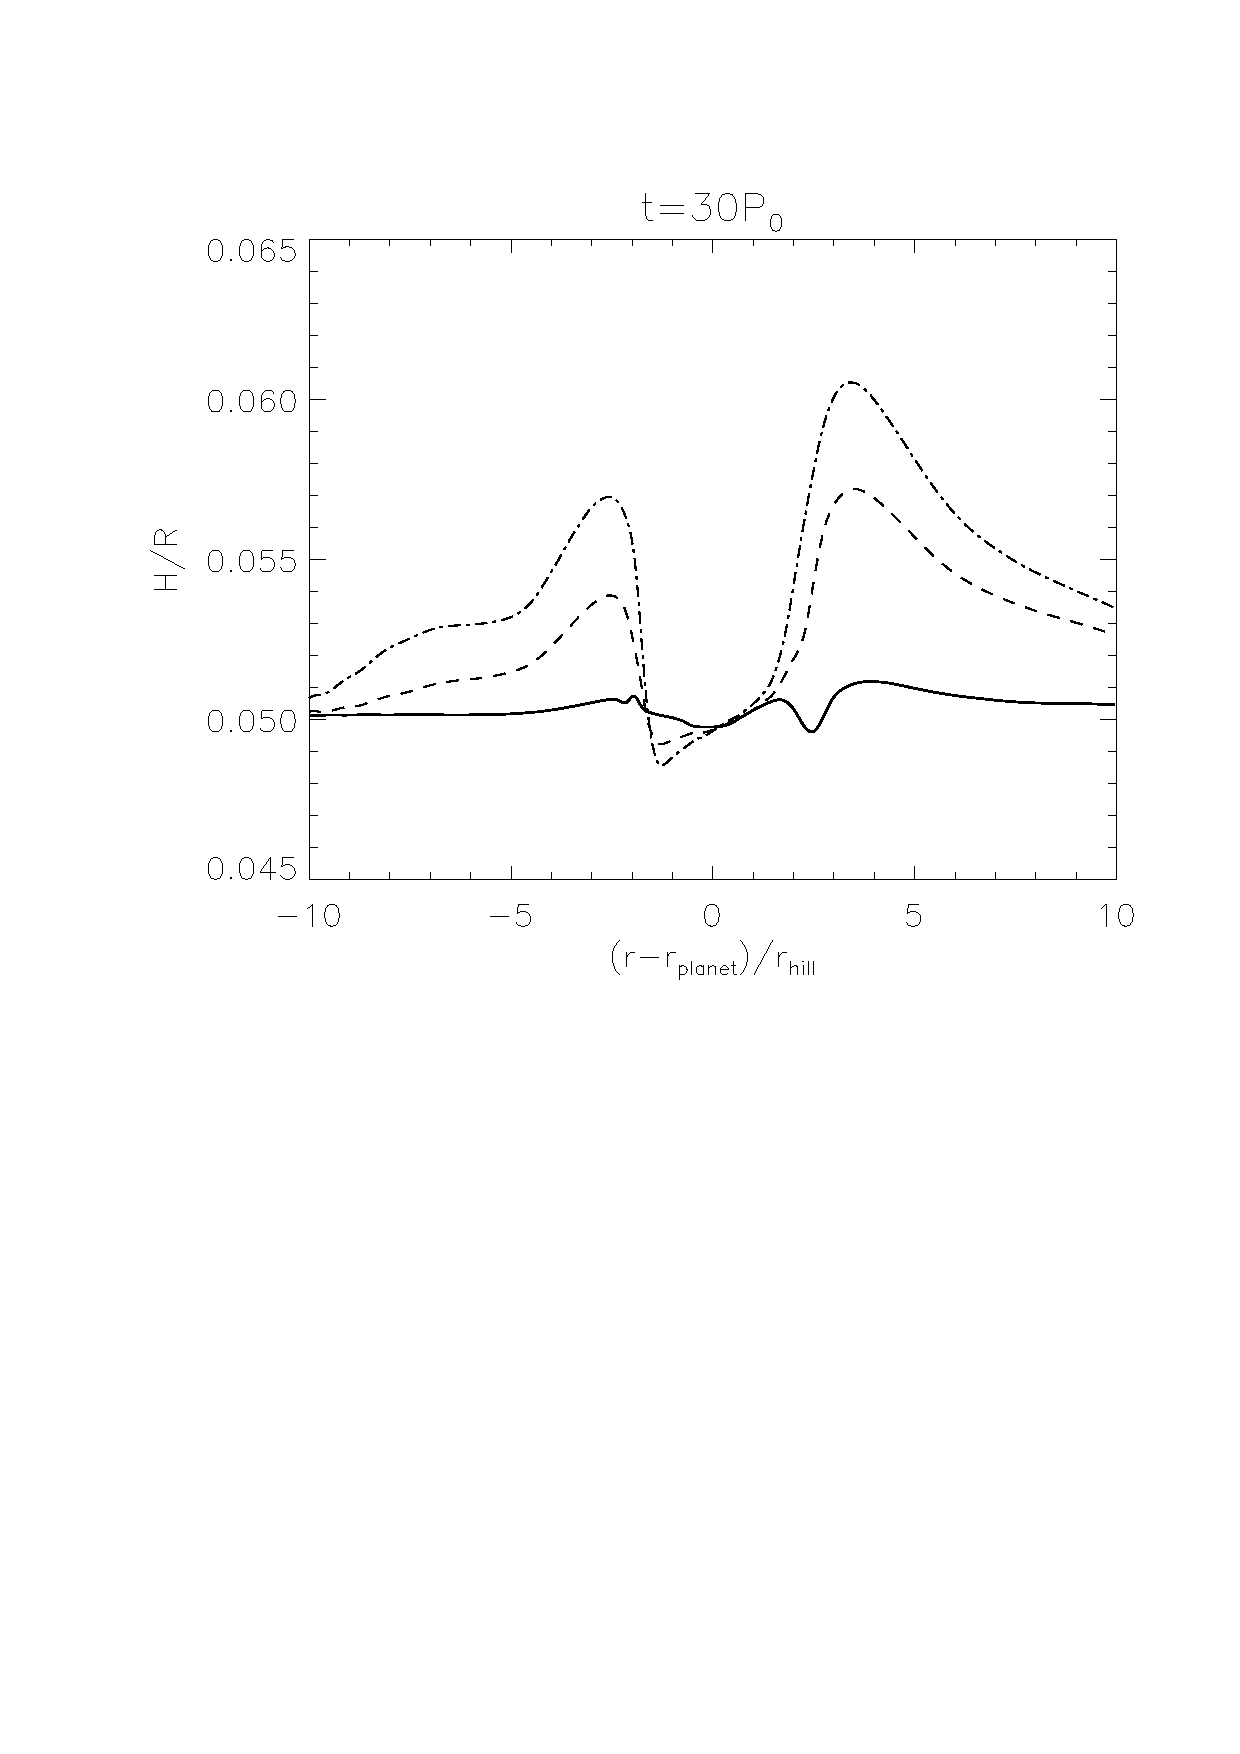
\includegraphics[width=\linewidth,clip=true,trim=0.5cm
    2cm 0cm 1cm]{figures/compare_aspectratio}
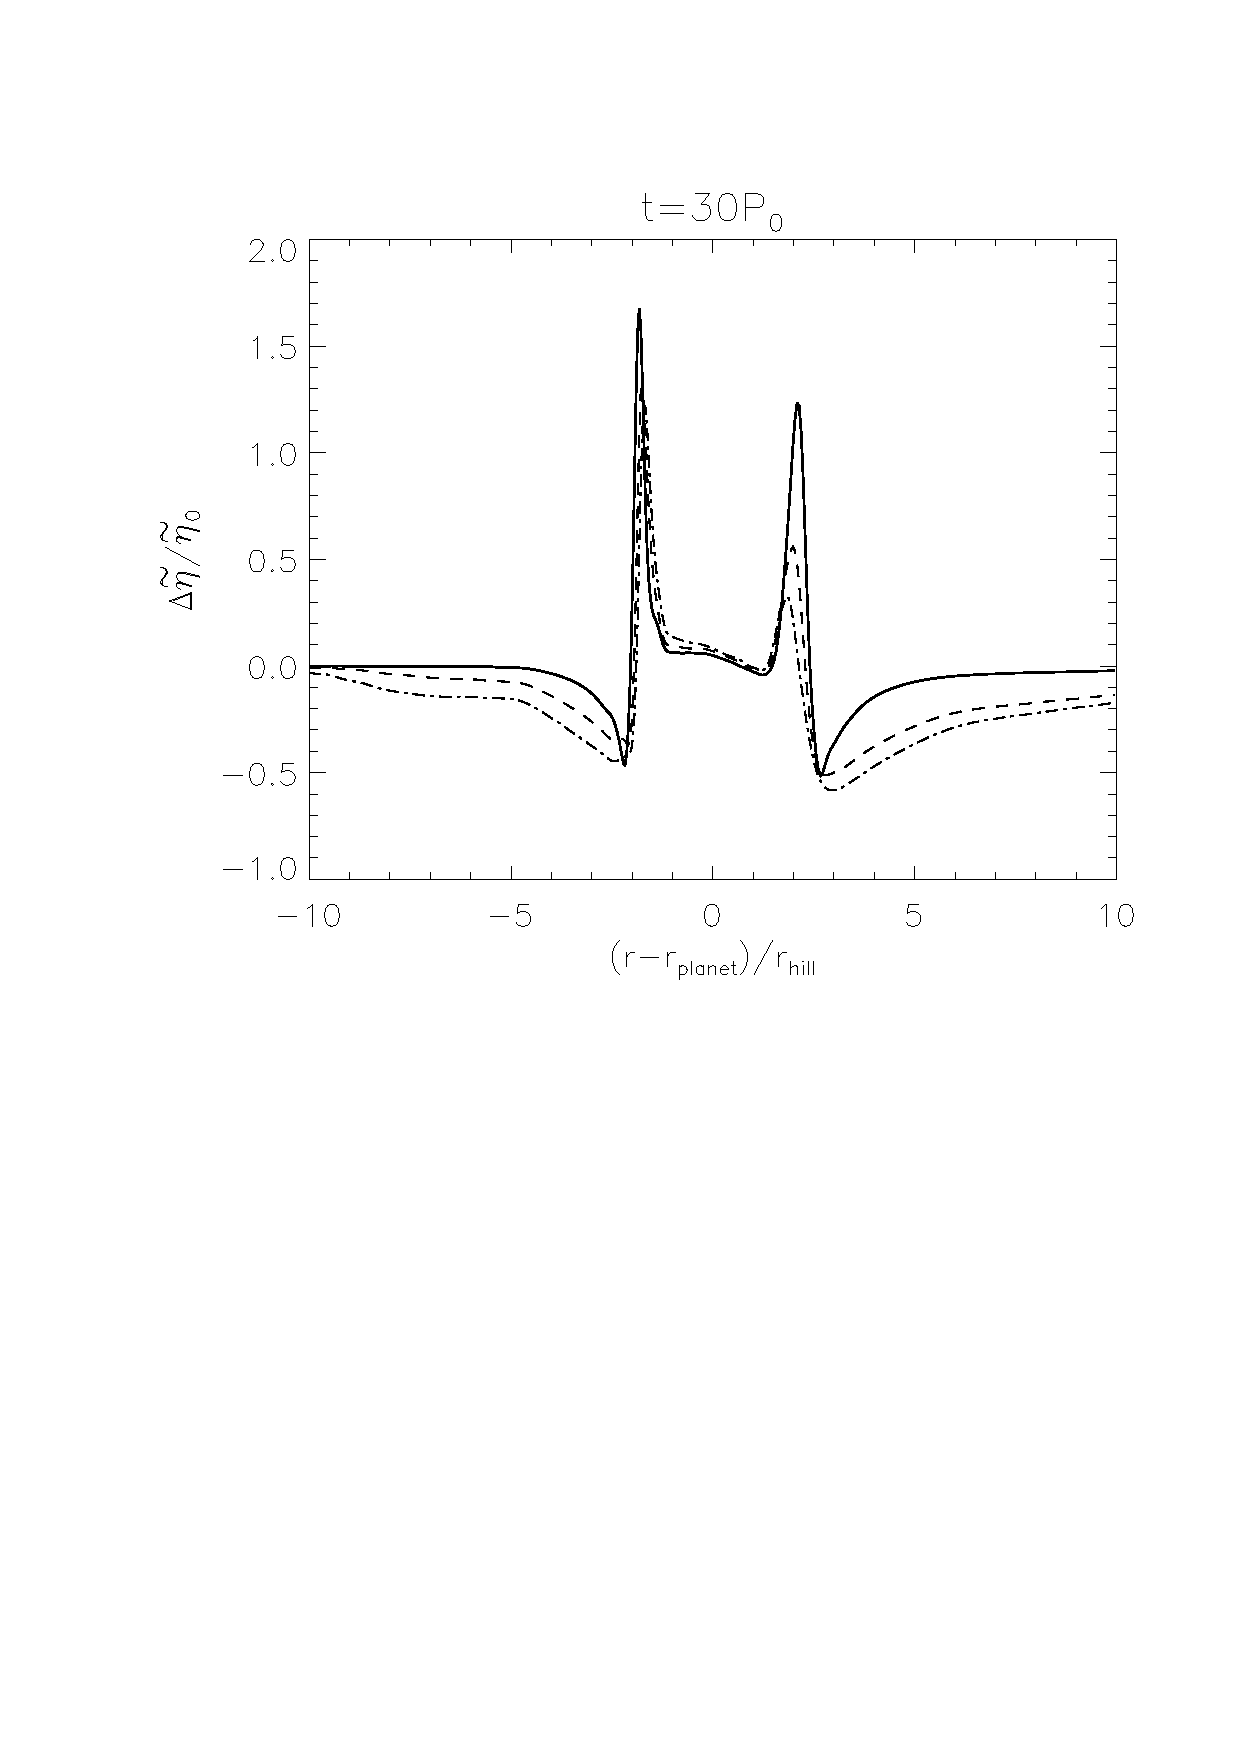
\includegraphics[width=\linewidth,clip=true,trim=0.5cm
    0.5cm 0cm 1cm]{figures/compare_gvortensity}
  \caption{Gap profiles at $t=30P_0$ for the intial partial gap opened
    before instability emerges for fast (solid), moderate
    (dashed), and slow cooling (dashed-dot). The relative surface density
    pertibation (top), disc aspectratio (middle) and generalized
    vortensity pertibation (bottom) are shown. \label{intial1D}}  
\end{figure}


%\begin{tabularx}{0.4\textwidth}{l*{10}{R}} \toprule
%  \multicolumn{11}{c}{$\tilde{\beta}=0.1$} \\ \midrule
%  m                    & 1 & 2 & 3 & 4 & 5 & 6 & 7 & 8 & 9 & 10  \\ 
 % $\gamma10^2/\Omega(r_o)$ & 6.56 & 6.82 & 6.73 & 5.78 & 6.00 & 6.38 & 5.97 & 5.62 & 4.61 & 3.36   \\ \bottomrule
%\end{tabularx}

%\begin{tabularx}{0.4\textwidth}{l*{5}{R}} \toprule
%  \multicolumn{6}{c}{$\tilde{\beta}=1.0$} \\ \midrule
%  m                    & 1 & 2 & 3 & 4 & 5  \\ 
%  $\gamma10^2/\Omega(r_o)$ & 1.27 & 1.28 & 1.35 & 1.01 & 0.61   \\ \bottomrule
%\end{tabularx}

\begin{table}
  \centering
  \caption{Dominant mode and growth rates for
    $\tilde{\beta}=0.1,1.0,10.0$ (fast, moderate, and slow cooling)
    values during `planet-off' simulations \label{modetable}} 
  \hfill
  \begin{minipage}{0.3\linewidth}
    \begin{tabularx}{\textwidth}{l R} 
      \multicolumn{2}{c}{$\tilde{\beta}=0.1$} \\ 
      \toprule
      $m$ & $10^2\gamma/\Omega(r_p)$ \\
      \midrule
      6 & 7.3 \\
      7 & 7.8 \\
      8 & 7.9 \\
      9 & 7.9 \\
      10 & 6.8 \\ 
      \bottomrule
    \end{tabularx}
  \end{minipage}
  \hfill
  \begin{minipage}{0.3\linewidth}
    \begin{tabularx}{\textwidth}{l R} 
      \multicolumn{2}{c}{$\tilde{\beta}=1.0$} \\ 
      \toprule
      $m$ & $10^2\gamma/\Omega(r_p)$ \\
      \midrule
      3 & 2.0 \\
      4 & 2.2 \\
      5 & 2.3 \\
      6 & 1.6 \\
      7 & 1.1 \\ 
      \bottomrule
    \end{tabularx}
  \end{minipage}
  \hfill
  \begin{minipage}{0.3\linewidth}
    \begin{tabularx}{\textwidth}{l R} 
      \multicolumn{2}{c}{$\tilde{\beta}=10.0$} \\ 
      \toprule
      $m$ & $10^2\gamma/\Omega(r_p)$ \\
      \midrule
      1 & 1.1 \\
      2 & 1.6 \\
      3 & 1.7 \\
      4 & 1.2 \\
      5 & 0.1 \\ 
      \bottomrule
    \end{tabularx}
  \end{minipage}
  \hfill
\end{table}

{\bf
\subsection{Axisymmetric stability}
Check that the gap profiles are stable against axisymmetric
stability. Can use analytical criteria given in section 3.1 of Li et
al (2000, ApJ, 533, 1023). No plot needed, just statements. 
}

The intial planet-disk interaction form bumps and grooves in the gap profiles
 which can potentially be unstable due to axisymmetric instabilities. The
 generalized local axisymmetric stability condition is the Solberg-Hoiland
 criterion,
\begin{equation}
 \kappa^2+N^2 \geq 0 $ where $ N^2=\frac{1}{\Sigma} \frac{\partial P}{\partial r} \left(\frac{1}{\Sigma} \frac{\partial \Sigma}{\partial r}-\frac{1}{\gamma P} \frac{\partial P}{\partial r}  \right)
\end{equation}
where $N$ is the Brunt-V\"ais\"al\"a frequency for the disk due to entropy
 variation which is non-zero for non-adiabatic models such as being considered.
 At  $t=30P_0$ the outer gap edge of $r=2.5r_h$,  where the RWI is excited the
 criterion value, is found to be approximately $0.002$ for all $\tilde\beta$
 which is the local minimum in the gap region which indicates local
 axisymmetric stability of gap. The Solberg-Hoiland criteria is similary
 satisfied for the entire disk and for all times within the simulation length
 with little change of values. Thus for all cases of $\tilde\beta$ the
 planet-induced gaps formed are stable to axisymmertic instabilities.

\subsection{Non-axisymmetric instability}\label{linear}
%{\bf present `planet-off' simulations. one `fourier mode v.s. time'
%  plot to show growth of linear instability. do an adiabatic case (or
%  extremely long cooling time) to see the effect of heated gap edge
%  (i.e. temp doesn't go back to t=0 value too quickly)
%  compare growth rate and dominant
%  m as function of beta (table). 2D figs to contrast (also used to
%  show it's the minimum in generalized pv that goes unstable.    
%  result: increasing cooling time makes the gap
%  more stable, and favors lower m. note: the `basic state' should be
%  the system at t=30 after azimuthal average. linear results should
%  have small perturbations. 
%}

%After the azimuthal averaging, the small pertibation excites rapidly
%growing instabilities by the RWI. 

In all cases we observe growth of non-axisymmetric structures after the
planet potential is switched off and the system subject to random
perturbations. An example is shown in Fig. \ref{linearmodes} for 
$\tilde{\beta}=10$. We charcterize these
modes with an azimuthal wavenumber $m$ and growth rate $\gamma(m)$ as defined by
Eq.~\ref{fouriertransform}---\ref{growth} with radial range of $[2r_h,5r_h]$. Table \ref{modetable}
lists the growth rates for the three cooling
times, measured during linear growth. 


\begin{figure}
  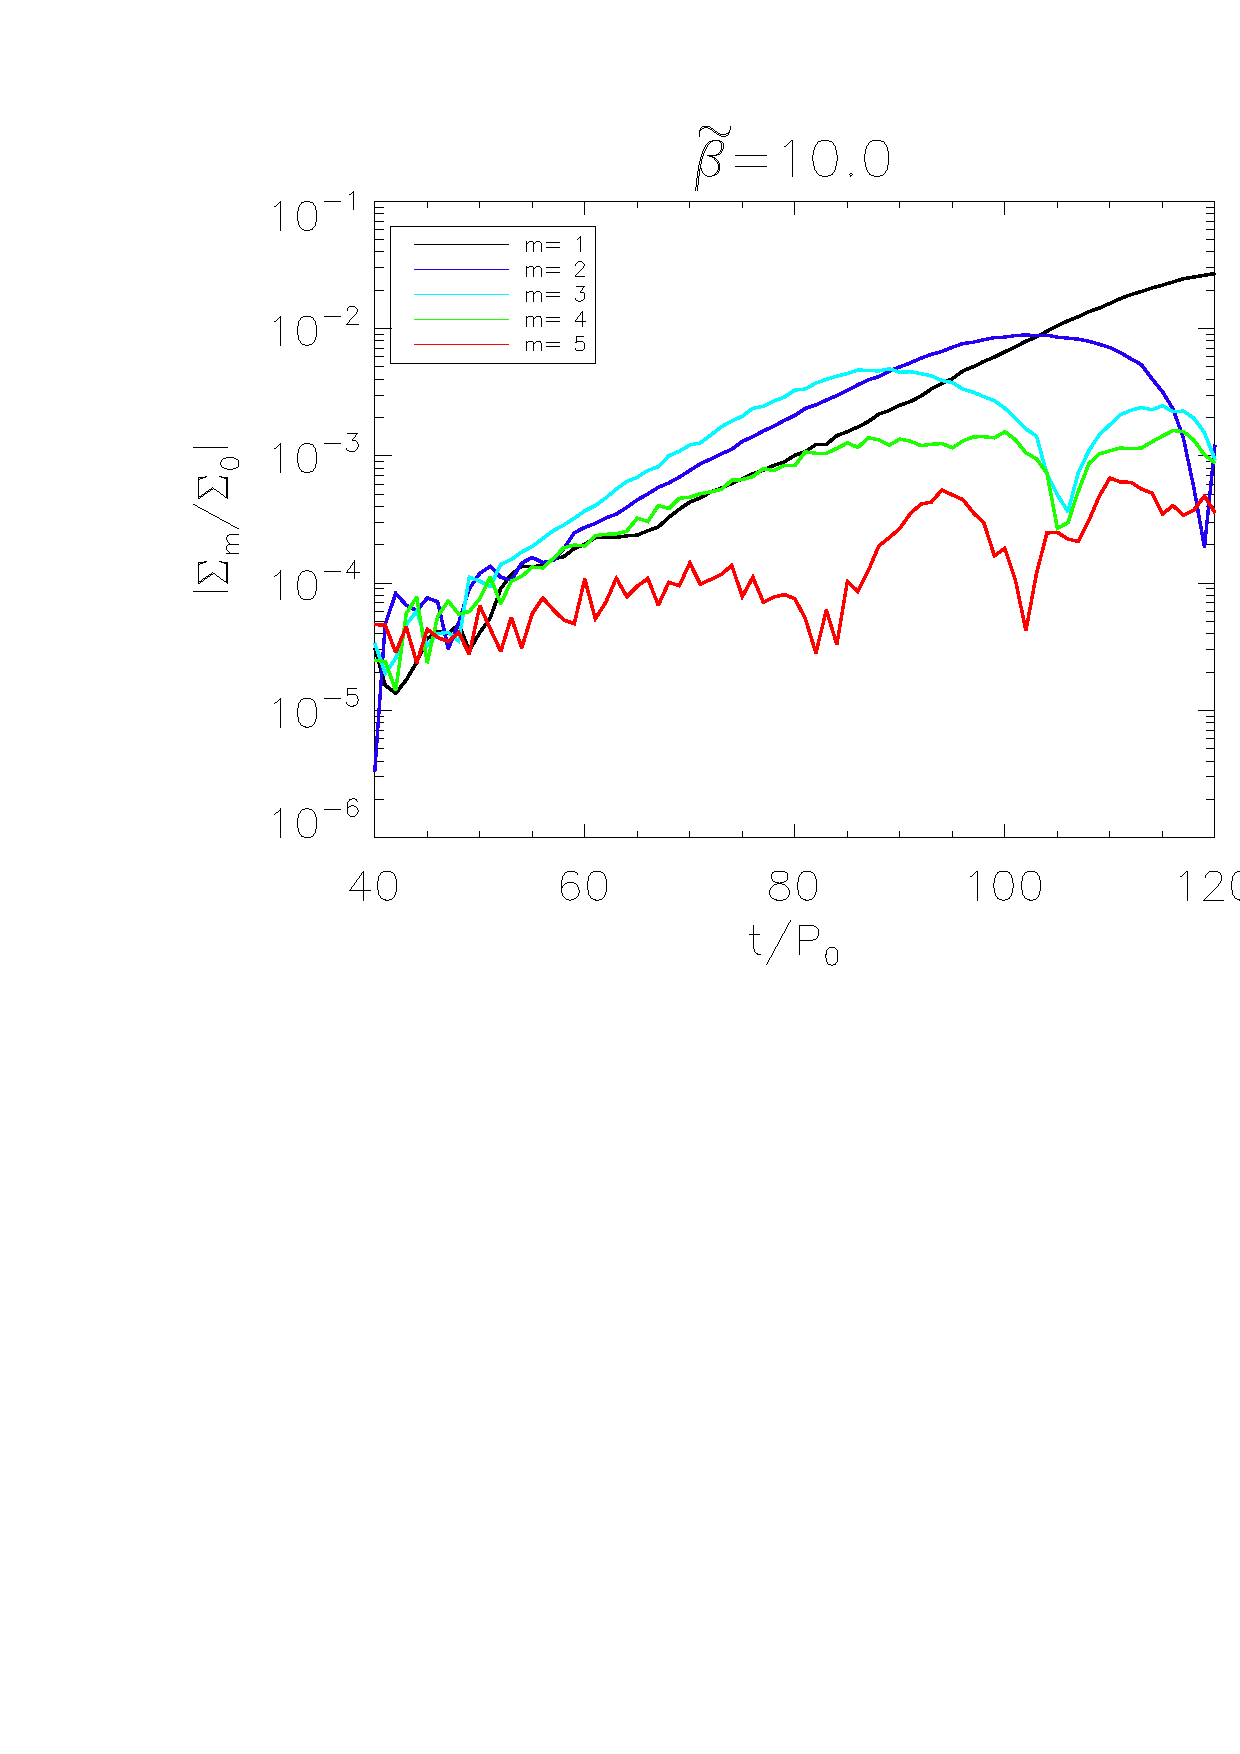
\includegraphics[width=\linewidth,clip=true,trim=1.2cm
    0cm 0cm 0cm]{figures/linear_stability}
  \caption{Evolution of azimuthal Fourier modes of disc surface
    density, non-dimenionlized by the axisymmetric background keplerian mode
 $\Sigma_0(t=0)$ for the
    `planet-off' simulations with $\tilde{\beta}=10$. Colours correspond
    to different $m$ values. The $m=3$ component is the fastest growing
    mode during linear growth and has a corresponding
    $\gamma=0.017\Omega(r_p)$.\label{linearmodes}}
% {\bf is the $\Sigma_0$ at t=0?} }  
\end{figure}

%%%%%%%%%%%%%%%%%%%%%%%%%%%%%%%%%%%%%%%%%%%%%%%%%%%%%%%%%%%%%%%%%%%%%%%

Table \ref{modetable} show that as
$\tilde{\beta}$ was increased from $ 0.1\rightarrow10$ the dominant
azimuthal Fourier mode decreased from $ m=9\rightarrow3$ and the
respective growth rate decreased from $ \gamma/\Omega(r_p)=0.079
\rightarrow 0.017$. However, despite two orders of magnitude increase in the
cooling time, the instability remains dynamical with growth time
$\lesssim 10P_0$. Snapshots of the instability in $r-\phi$ plane for
the different $\tilde\beta$ are shown in Fig \ref{2Dlinear}. 

These `planet-off' simulations show that gap edges become more stable with
longer cooling times. This is expected because larger $\tilde{\beta}$
result in hotter gap profiles at $t=30P_0$ with less pronounced
generalized vortensity minima. Stabilization with increased
cooling time is therefore due to a smoother basic state for the
instability, as it is more difficult for the planet to open a gap if
the disc is allowed to heat up. 
 

% which result in hotter gaps since the heating
%due
%This is as expected from the
%intial gap profiles, because 
% and the gap forming criteria discussed in the
%previous section. 





\begin{figure}
  \centering
  \subfigure{
    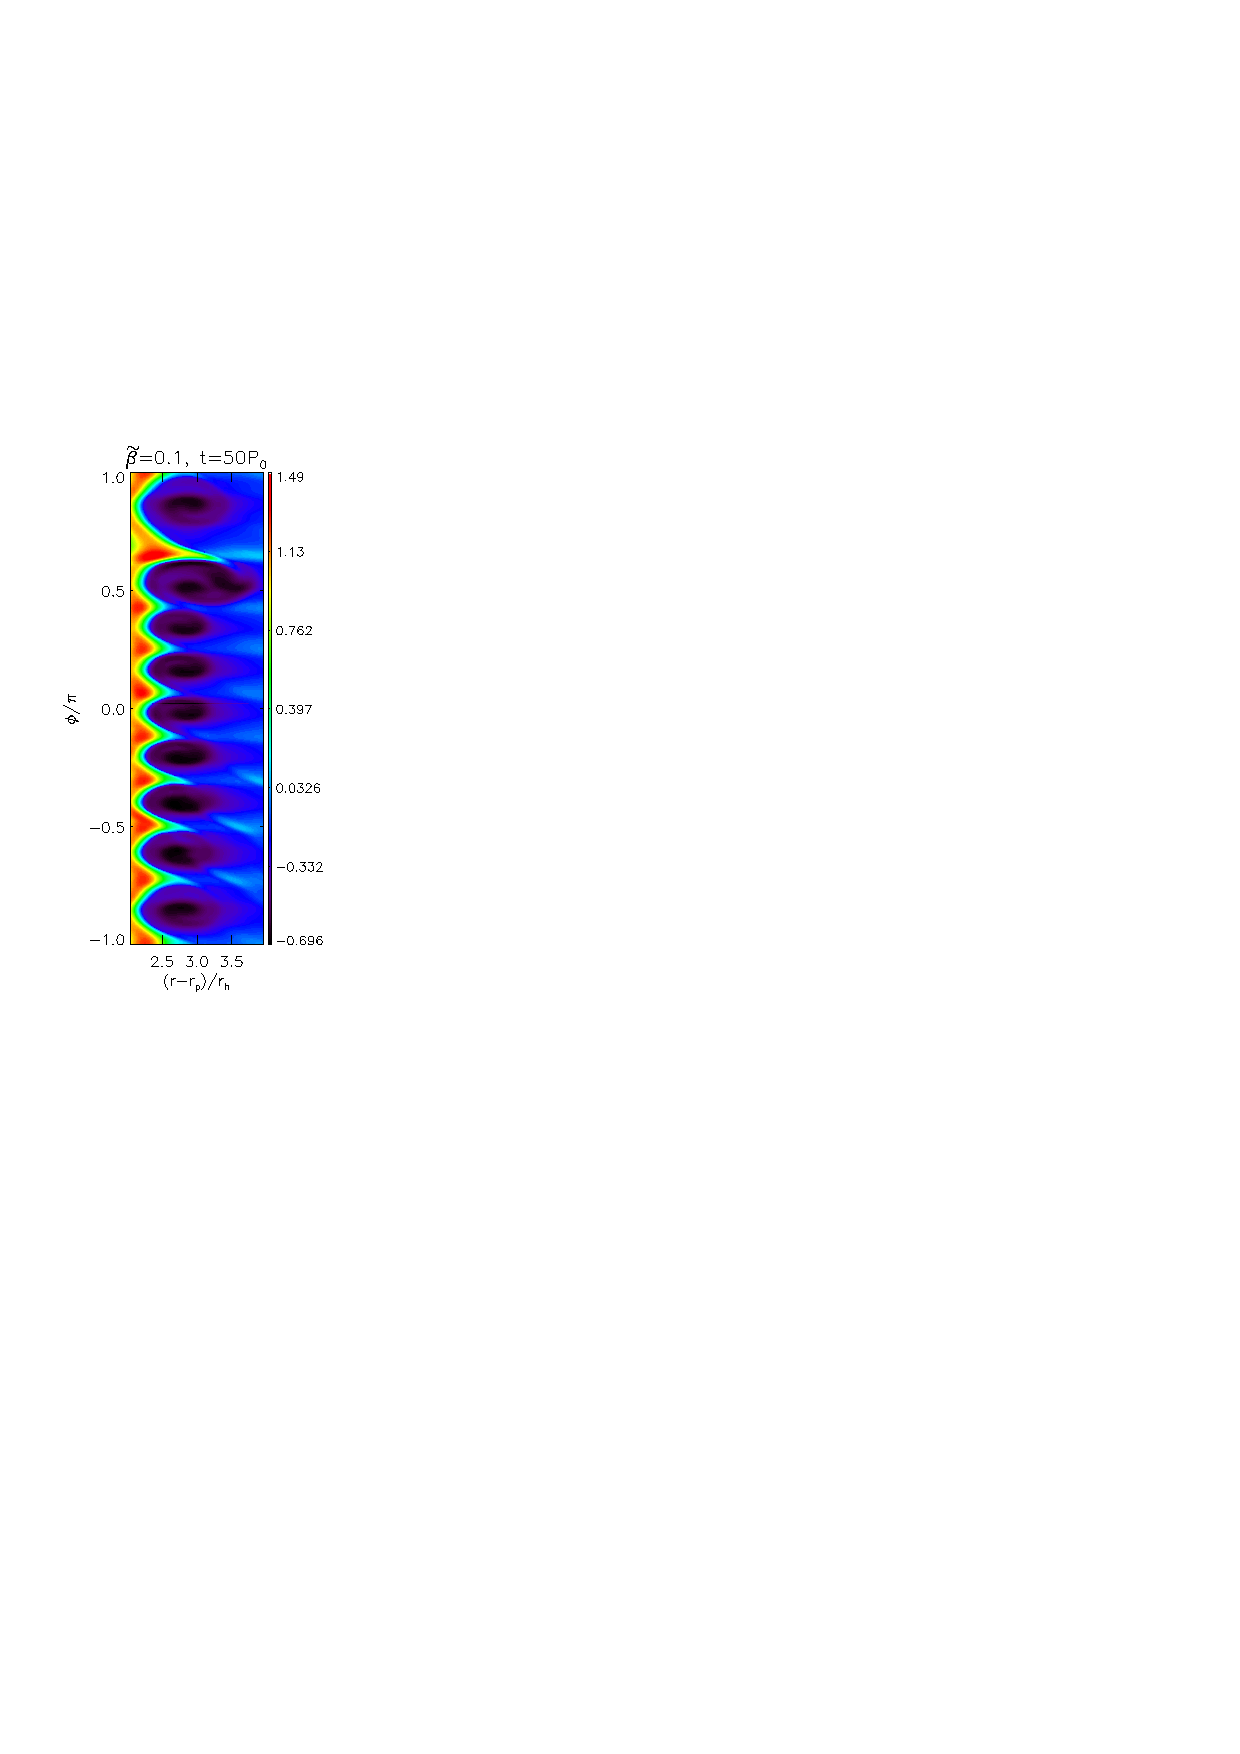
\includegraphics[width=0.3\linewidth]{figures/analysis_gvortensity50}
  }
\hfill
  \subfigure{
    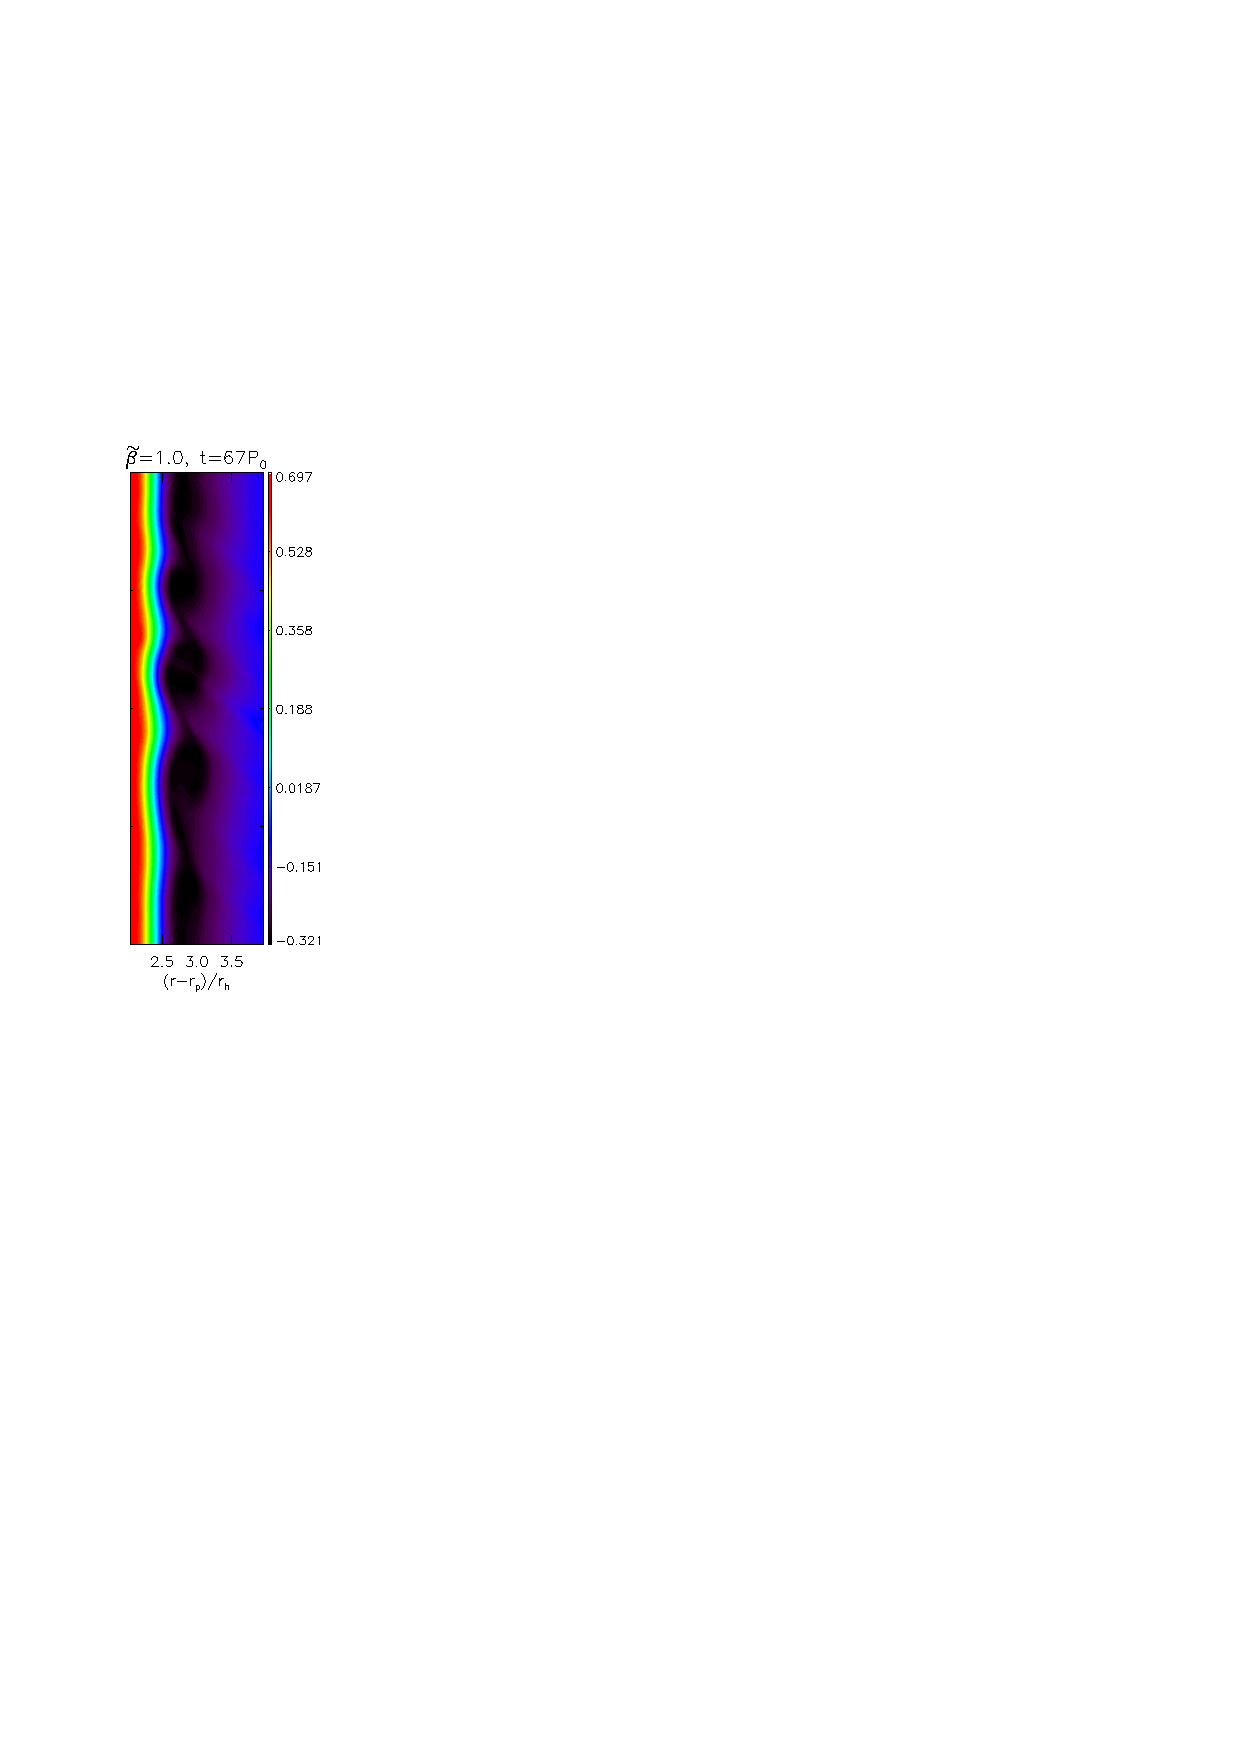
\includegraphics[width=0.3\linewidth]{figures/analysis_gvortensity67}
  }
\hfill
  \subfigure{
    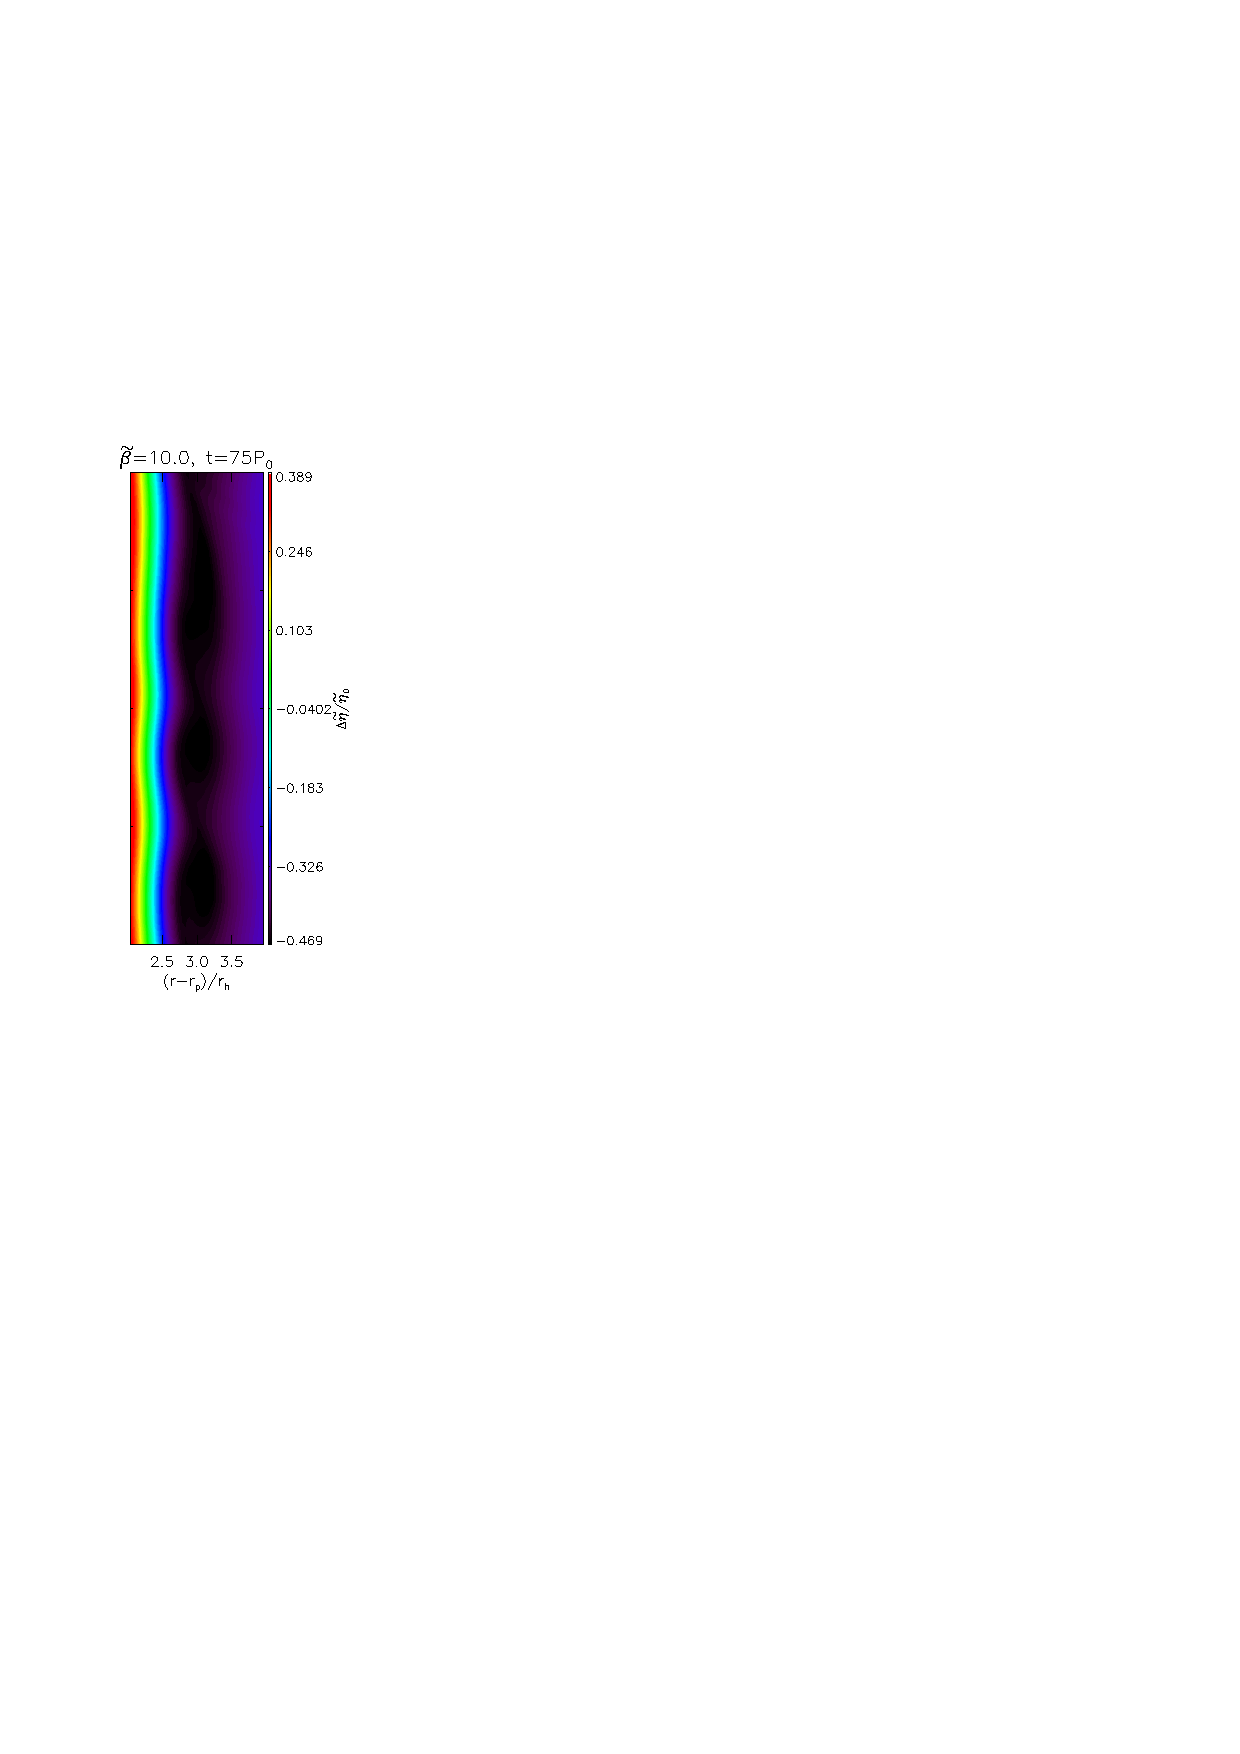
\includegraphics[width=0.3\linewidth]{figures/analysis_gvortensity75}
  }  
  \caption{Generalized vortensity perturbation (relative to $t=0$) for
    cases of $\tilde{\beta}=0.1,1,10$ (left,middle,right) during
    the growth of non-axisymmetric modes. The planet potential has
    been switched off.  The number of vortices
    decrease as $\tilde{\beta}$ increases. Note that snapshots are
    taken later because it takes longer for the vortices to grow and
    become visible with increasing cooling time. 
    %    correspondingly increase to capture the longer growth phases of
    %    the instabilities. 
    \label{2Dlinear} {\bf I'm curious to know if plots clearer if
      perturbations are measured relative to t=30? remember t=30 is
      our reference state for instability. But we'll probably keep
      these for consistency (later non-linear plots are all measure
      with respect to t=0).}} 
\end{figure}

\subsubsection{Nearly adiabatic discs}
\label{adiabatic_section}
%{\bf a case with extrmely long cooling time (or adiabatic run) in
%  order to look at effect of heated gap edge.  prelim result: not
%  important, at t=30, gap edge only heats to $H/r\simeq0.06$ even for
%  purely adiabatic disk. change in $h$ not important for linear
%  perturbations (but important for setting up the basic state). 
%}
The above `planet-off' simulations are not formally linear
stability calculations, because the cooling time is shorter
than the instability growth time, 
%
%as we do not capture the effects of a heated
%disk on the instability growth. 
$t_c<\gamma^{-1}$.  
Thus the disk cools back to its intial value of $h=0.05$
before or during the instability growth, implying we do not have a
steady basic state to formulate a standard linear stability
problem. %This means the disc temperture of $h=0.05$ in the the above cases 

In order to perform a proper linear stability analysis and capture the
effect of a heated gap edge during instability growth, we ran a simulation  with
$\tilde{\beta}=100$, corresponding to an almost adiabtaic disc.  
%To compare our 'planet-off' analysis with a true
%linear stability analysis 
In this simulation the cooling rate is slow enough that the gap 
temperature profile (e.g. middle panel of Fig. \ref{intial1D}) changes
only marginally over the instability growth timescale. %heat is
                                %retained/maintained.   

We find very similar gap profiles and mode growth rates for
$\tilde{\beta}=100$ as with $\tilde{\beta}=10$. The disc heats up to
values $h\simeq0.06$ in the nearly adiabatic case. This is close to
the original temperature of $h=0.05$, so linear growth rates are not expected
to change significantly %according to the linear theory presented in
\citep{li00}. 

According to \cite{li00}, increasing $h$ increases linear growth rates
of the RWI because it is pressure-driven. However, in the case 
of disc-planet interaction, increasing $h$ has a stabilizing effect
through the gap profile because it results in smoother gap
edges. The fact that we observe smaller growth rates as $h$ is
increased indicate that for planetary gaps, the importance of $h$ on
the \emph{linear} RWI is through the setting the gap profile (i.e. basic
state for the instability). 



%results in shallower gaps
%which is expected to be  

%the difference in growth rates between this and the
%original disc temperature of $h=0.05$ changes almost insignificantly
%as shown by linear theory \citep{li00}. 
%Although linear
%theory predicts higher growth rates with increasing $h$ 

%This indicate that a
%continuously hot gap edge is not as important for development of
%vortices as the heating effects on the formation of the intial gap
%state. 


%{\bf
%If there's time, do low resolution planet off simulations but keep the planet on
%until $t=40P_0$ or $50P_0$. Look at stability properties when the gaps
%are generally deeper (including the nearly adiabatic case). Although
%with the planet instability may already appear by $t=40P_0$, the
%azimtuhal average performed prior to perturbations will erase it.}



%%%%%%%%%%%%%%%%%%%%%%%%%%%%%%%%%%%%%%%%%%%%%%%%%%%%%%%%%%%%%%%%%%%%%

\section{Non-linear evolution of
  gap-edge vortices with finite cooling time}\label{nonlinear} 
%{\bf main fig: vortex amplitude v.s. time for diff beta. enough data
%  to plot vortex lifetime v.s. beta? table: 
%  averaged quantities over quasi-steady state: aspect-ratio (to
%  compare with fu at al), rossby number (vortex strength
%  v.s. cooling?), maybe alpha visc. vortex size: visible difference?  
%  only inviscid cases. describe evolution of one case. main
%  conclusion: longer vortex lifetime with increasing cooling time (up
%  to some optimal timescale). vortex death: induced-shock and/or
%  smoothing the gap edge. describe simulation setup, resolution?
%  should mention that results consistent with lower-resolution prelim
%  runs. maybe torques? 
%}

We now consider long term simulations of gap-edge vortices for
$\tilde{\beta}=0.1,0.5,1,5,10$. The planet potential is kept on
throughout.  
% up to a total of
%$2000P_0$. 
%Planets were left free to interact dynamiclly with the disk
%and vortices after $t=30P_0$ as apposed to previous section.  
We employ a grid with $(N_r,N_{\phi})=(512,1024)$ 
in order for these simulations to be computationally feasible. We also use a larger
disc with $r_{\mathrm{out}}=45r_{\mathrm{in}}$ to minimize boundary
effects on vortex evolution. We apply an open boundary at
$r_\mathrm{out}$.

Preliminary simulations with same numerical scheme but lower resolution of
 $(N_r,N_{\phi})=(256,512)$ where also done for the above $\tilde\beta$ values
with the inclusions of $\tilde{\beta}=0.25,0.75,2.5,7.5$ as well.
Results and vortex behaviour are convergent with
higher resolution simulations as discussed in this section.
 {\bf mention lower resolution preliminary runs -
  similar results to those presented here (?). want to demonstrate convergence}



%An open boundry
%condition was used in the outer edge of
% allowing significant room for
%linblad resonances of the vortices. 


\subsection{Generic evolution}

The linear growth of the RWI and vortex-formation is followed by 
vortex merging. Merging timescales are independent of $\tilde\beta$ value,
 and by $60P_o$ only one vortex remains as the growth of these modes are now
 accelerated by planetary influence.
%i.e. only the $m=1$ mode remains. 

The evolution of the amplitude of the $m=1$ surface density mode
 over the radial range of $[2r_h,10r_h]$ is shown in Fig~\ref{lifetimeplot}
 for different $\tilde\beta$.
% {\bf should state (also for planet-off runs)
 % what the radial range is used for averaging the Fourier amplitudes} 


\begin{figure}
  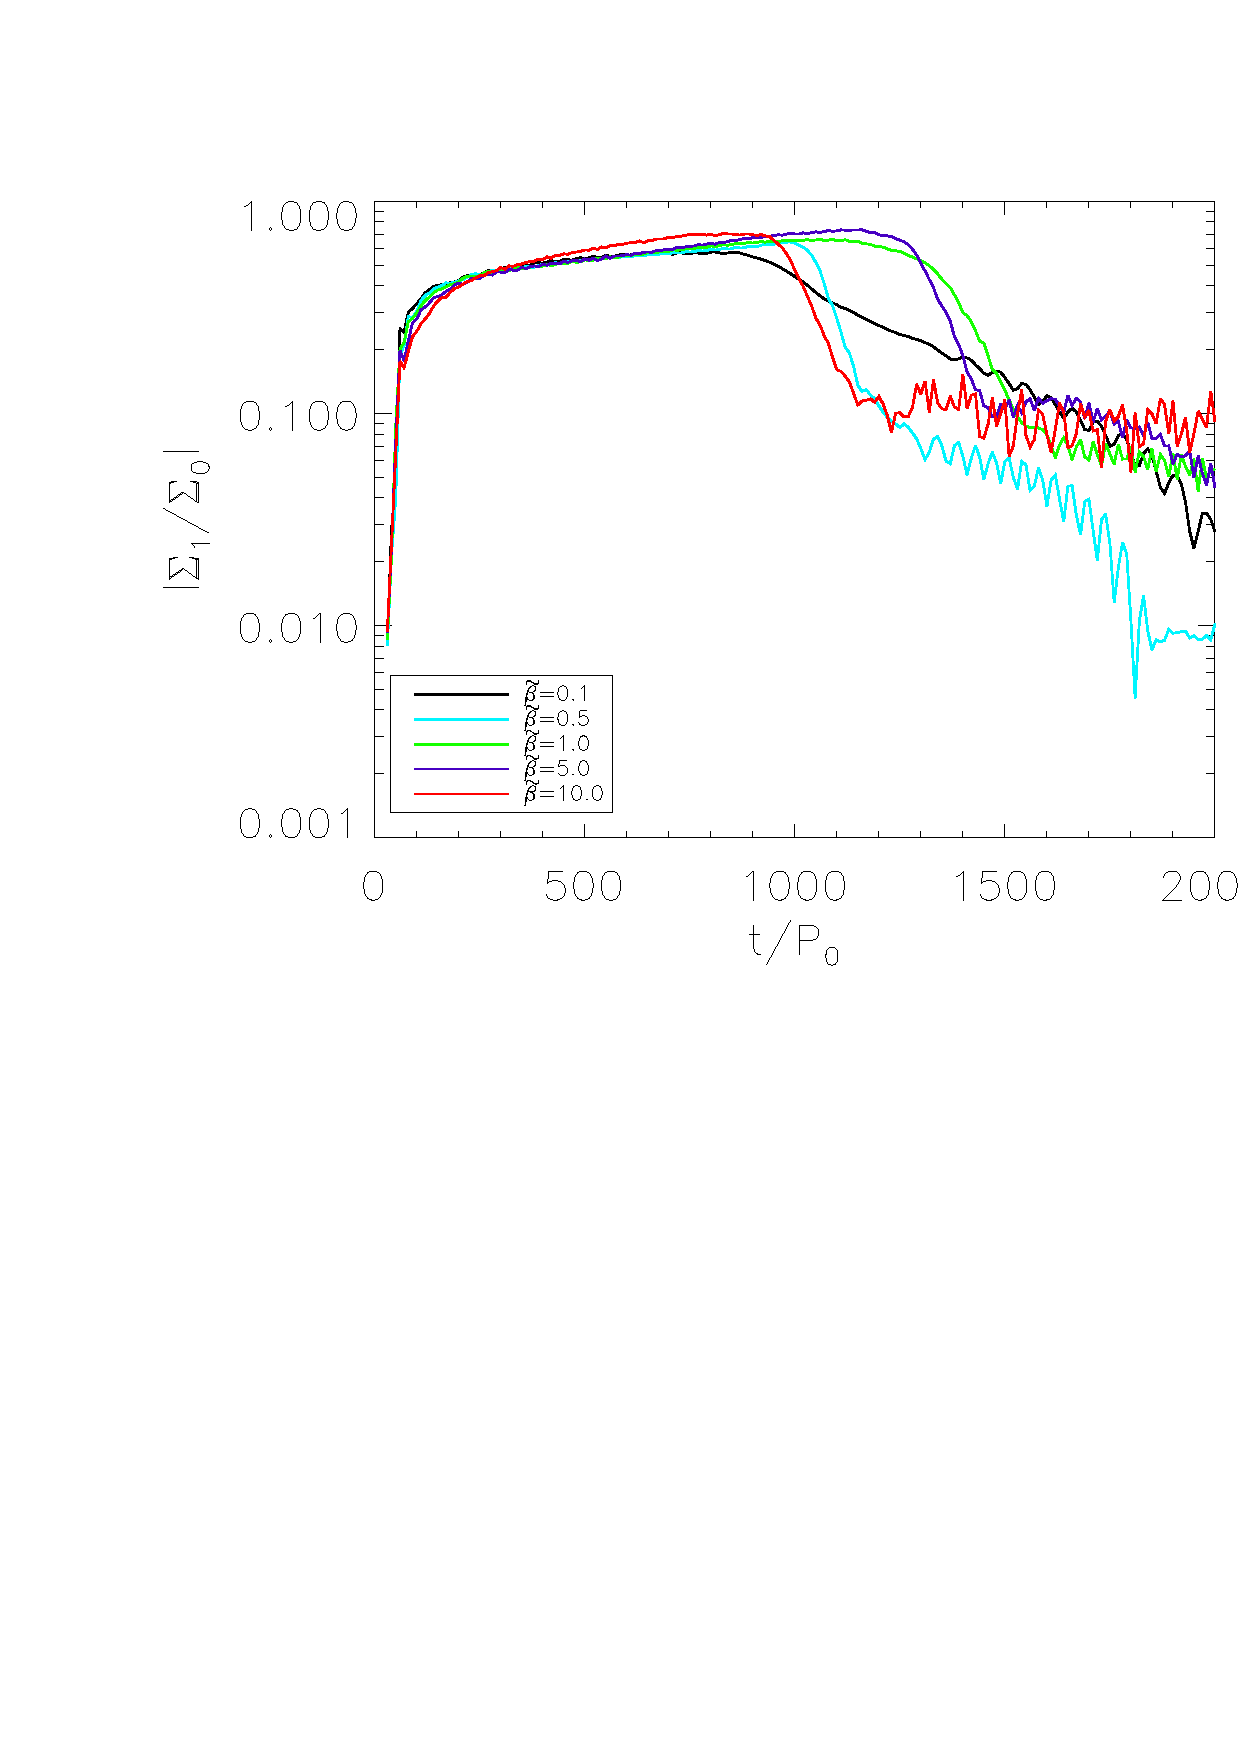
\includegraphics[width=\linewidth,clip=true,trim=0.5cm
    0cm 0cm 1cm]{figures/longterm_stability}
  \caption{Log plot of the $m=1$ mode non-dimenionlized by the $m=0$
    background mode for longterm non-linear simulations corrsponding
    to vortex lifetime. The longest living mode correpsonds to
    $\tilde\beta=5.0$ (the red line). \label{lifetimeplot}} 
\end{figure}

In all cases the system remains in a quasi-steady state for
$\gtrsim800P_0$ with a single vortex circulating 
the outer gap edge at the local Keplerian  
frequency. Fig. \ref{Vortex2D} shows a typical plot of the relative 
surface density perturbation in this state. During this stage, the 
vortex grows in intensity. As the vortex forms it has a
 value of $Ro\approx-0.1$ for all $\tilde\beta$
 indicating anti-cyclonic
motion. As the $m=1$ amplitude grows the relative spin of the vortex
continuously grows along with it, reaching values of
$Ro\approx-0.4$ characteristicly for all cooling rates. Relative surface
 density pertibations at the center of vortices can reach values of 7 times the
 intial density for all cases of $\tilde\beta$ in this quasi-steady state and
 can be found as high as 9 times for the $\tilde\beta=1.0$ case.
 The gap profiles apply a surface density boost in the vortex region as the
 vortices are located at the gap edge maxima
 but the values associated with this boost have relative density pertibations
 of under 1 and thus are negligibe compared to the max amplitudes of the vortices.
 Vortex growth is attributed to
the continuous generation of vorticity by the planet-disc interactions. 
This is supported by the evidence that in long term simulations where the
planet is removed such as in section \ref{nonlinearplanetoff} the amplitude of
 the vortices are not seen to contiunously grow without the planet influence.


{\bf is vortex merging affected by $\tilde{\beta}$? e.g. timescale
  taken to reach one vortex as a function of cooling}
{\bf for what cooling are these values quoted for? do
  these values depend on cooling?}
 {\bf is the evidence for this the fact that growth is not observed in
  planet-off simulations?}   

{\bf note that there
  are two origins for the surface density boost relative to $t=0$: 1) gap
  formation, which increases the surface density at the location of
  the instability (since they happen at surface density max., and 2)
  vortex instability). what is the surface density boost relative to
  the gap profile?}   


Interestingly, in most cases we observe a sudden drop in 
the $m=1$ amplitude within the simulation time, which occurs over
timescales of $t\in[20P_0,70P_0]$, i.e. much shorter than the duration of the
quasi-steady state. Dissipation timescales follow the basic trend of decreasing with increasing $\tilde\beta$ but more accurately correlated with Mach number values which will be discussed in following section
{\bf is this dissipation timescale independent of cooling? Trend is based on mach values which dont follow linear trend } 
%Eventually
%the $m=1$ amplitudes are also characterized by 
After these characteristic drops, the instability is never seen to
reform at such large overdensities and surface density bumps are never larger
than that due to the planetary wakes. We designate the time of these
amplitude drops as the lifetime 
of the quasi-steady vortex.
The instability is not seen to emerge again after the intial vortex dissipation
 due to the smoothening out of the gap edge during dissipation by the
 transfer of density from the once tightly held vortex region to the surrounding
 disk and gap.  
{\bf question: does instability
  actually happen again? if it does, but just weaker, that may be
  because the first vortex has smoothed out the gap edge, so
  instabilities following that would be weaker.}



\begin{figure}
  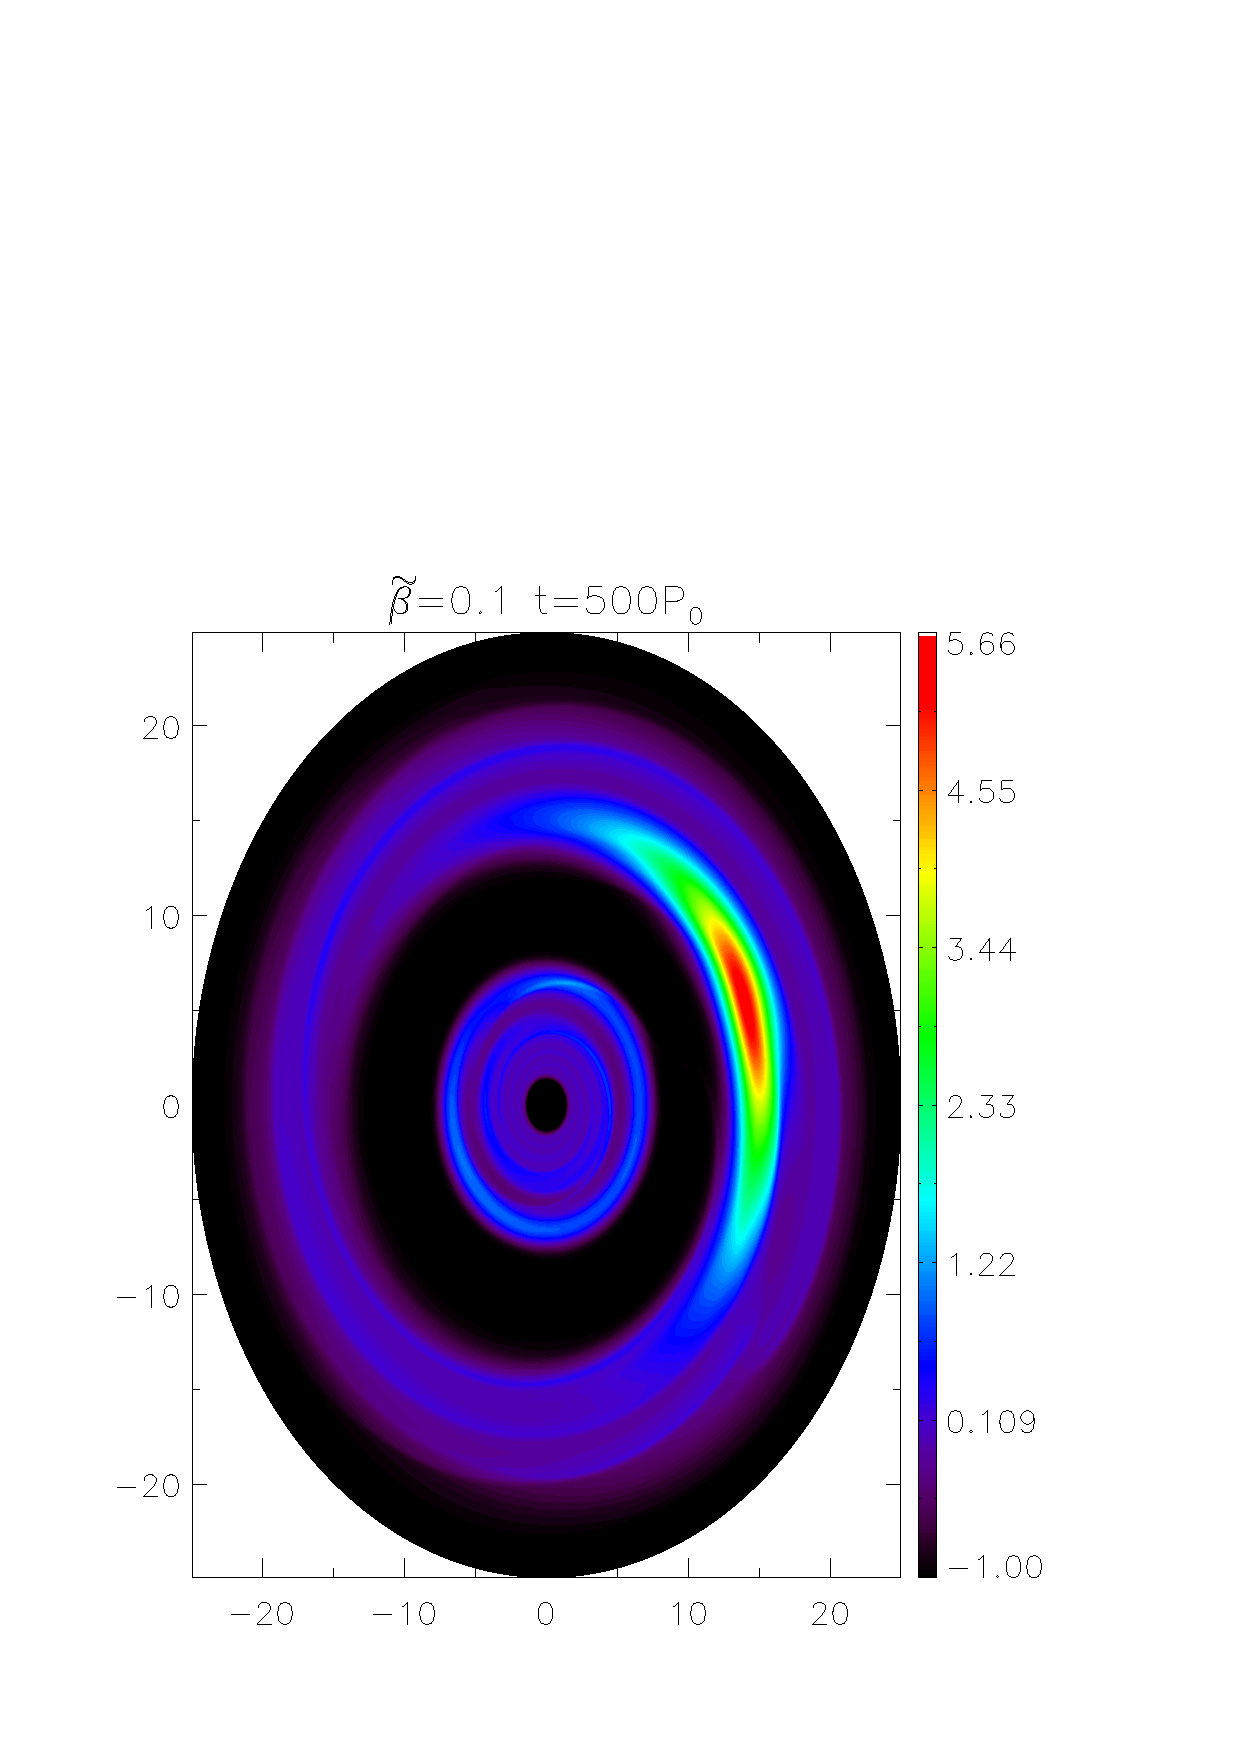
\includegraphics[width=\linewidth,height=\linewidth]{figures/vortex2D}
  \caption{Relative surface density perturbation for the
    $\tilde\beta=0.1$ case during quasi-steady state with a single
    vortex. The plot for other values of the cooling time $\tilde{\beta}$ are
    similar.% {\bf is this plot truncated? in the text it says the
      %domain goes to $r=45$?}
    %The large scale non-axisyemetric $m=1$ overdensity can be
    %seen. 
    \label{Vortex2D}} 
\end{figure}

\subsection{Non-linear instability without planet influence} \label{nonlinearplanetoff}
Non-linear observations were also made for the `planet-off' simulations.
After the linear growth phase of the vortices, vortex merging takes hold but
 now on timescales of up to $150P_0$ as the vortices grow as linear
 instabilities discussed previously. The vortex merging time is depedendent on
 the growth rates of the modes and how long they take to saturate. Similar
 quasi-steady vortices form but the long-term behaviour is significantly
 different without the planet as seen in Fig.\ref{planetofflifetimeplot}.
 The quasi-steady vortices formed have significantly lower density pertibations
 and now slowly decrease in amplitute in time as apposed to previously
 where their growth was supported by planet interactions. The vortices simply
 dissipate viscously and no longer undergo the quick dissipation that
 characterized the dissipation as earlier. The dissipation rate is dependent
 on the cooling rate with viscous dissipation decreasing with larger
$\tilde\beta$.

\begin{figure}
  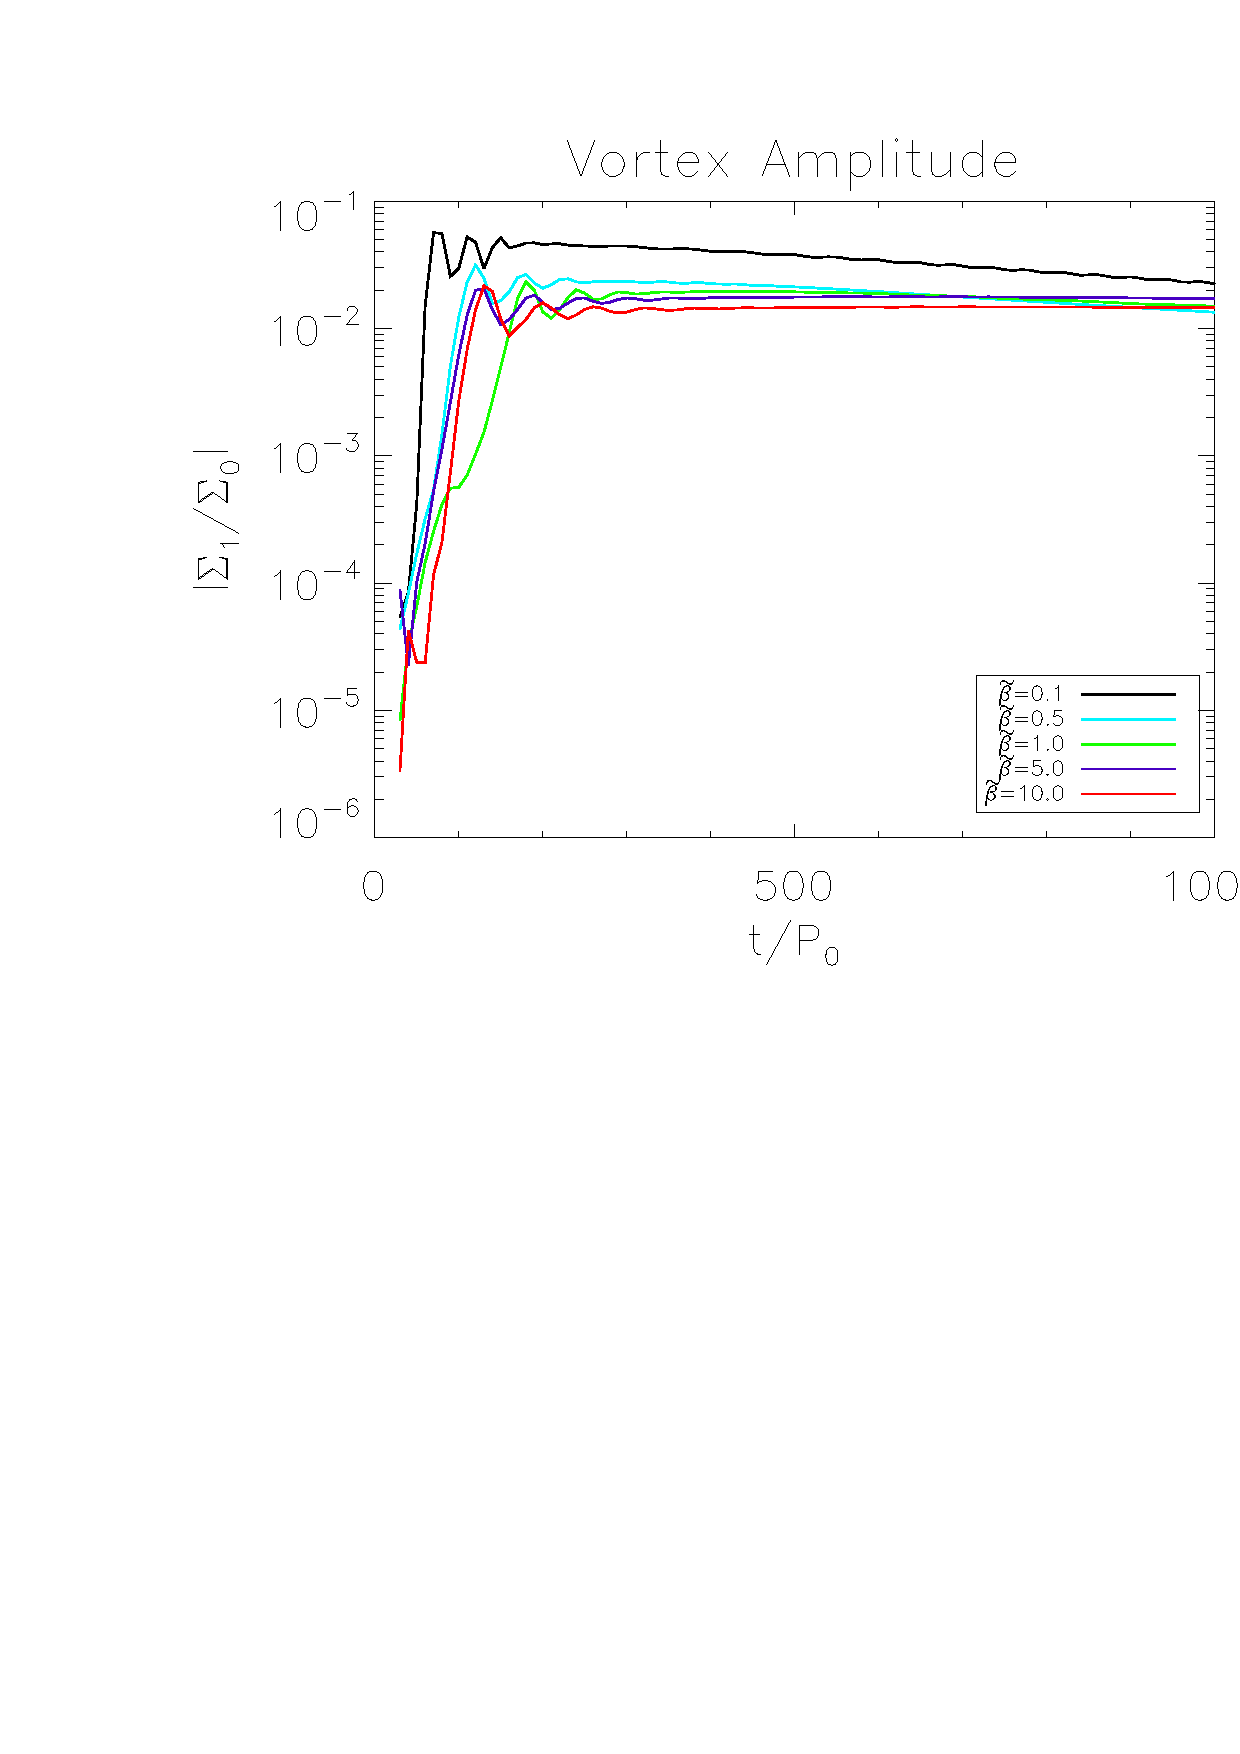
\includegraphics[width=\linewidth,clip=true,trim=0.5cm
    0cm 0cm 1.1cm]{figures/longterm_planetoff}
  \caption{Similar plot as Fig. \ref{lifetimeplot} but with `planet-off' simulations. Vortices dissipate viscously without planet driving influence} \label{planetofflifetimeplot}
\end{figure}

{\bf
\subsection{Additional analysis on vortex dissipation}
Conjecture: vortex death due to vortex shocking the system and
dissipating its energy. discuss one case. here we want to explain or
suggest why vortices die} 
%Rossby values have dynamics that are coupled with the lifetime and
%$m=1$ amplitude of the vortices. 

Gradients of surface density are seen to
spike up in wake-like features around the vortex during dissipation. 
Snapshots of relative density pertibation and density gradients during the
quasi steady state, during disspation and just before death are displayed in
Fig. \ref{shockplot} for $\tilde\beta=1.0$. Quasi-steady vortices have large 
elliptical shapes, while dissipating vortices are denser and smaller in spacial
extent.
As the vortices grow in intensity wakes are seen to extend from them. These
wakes correlate with large gradients in surface density and are first seen
when vortices are in the later half of their quasi steady states. During this
phase the average value of the gradients along the shock region are
$|\nabla\Sigma| \approx 4 \Sigma$. Just before the vortices start dissipation
this quantity sharply increases to a value of $ \approx6 \Sigma$ in which it
 remains during dissipation and rest of vortex lifetime.  
As the vortex dies off as described above its associated Rossby number quickly
approaches $0$.


In addition, we also observed large increases in the Mach number near
the vortex during dissipation, which indicate susceptibility to
shocks. Mach numbers with repect to the vortex bulk motion around the vortex
 region of $|r-r_{vortex}|<2H$, where $H$ denotes the gas scale height, is
 $\approx 0.8$ after the intial formation of the vortices for all
 $\tilde\beta$. During the quasi-steady state the Mach number increases at a
 steady rate with larger increases for lower $\tilde\beta$. Time values in
 which Mach numbers reach values of 1 approximately correlate with the start 
of dissipation and during dissipation values quickly increase to larger max values.
 Dissipation timescales correlate with 
Mach numbers reached during dissipation as the quickest dissipation occurs for 
$\tilde\beta=0.5$ which is on order of $70P_0$ and reaches Mach number
 $\approx1.2$ while the $\tilde\beta=0.1$ case which dissipates on scales o
f $20P_0$ reaches Mach numbers $\approx1.4$
Thus, the sudden drop in vortex amplitude may  
be a result of the development of associated spiral shocks dissipating
its energy \citep[cf.][who 
  suggested damping due to planet-induced shocks]{fu14}.  

{\bf note that fu et al suggested vortex damping by the planet
  shocks. here, we are suggesting vortex dissipates energy by shocking
  the disk. our evidence is that we observe vortex growth before it
  dissipates, and spiral shocks associated with the vortex always
  develop before vortex death. once it starts shocking the disc it
  loses energy. if the planet-induced shocks were responsible, death
  should be more gradual. can we think of other evidences that it's
  not the planet shock that's responsible?}
{\bf show
  this. e.g. vortex before, during and after death. maybe show
  snapshots of surface density perturbation (vortex) compared with
  $\nabla\Sigma/\Sigma$ (vortex shocks). demonstrate vortex shape
  changes and shocks develop prior ot death. state whether this is
  generic for all coolings}. 
{\bf show mach number plot, or quote values. relevant mach
  number is fluid flow speed with respect to 
  vortex bulk motion around the disc. does the typical mach number
  near the vortex just before its death depend on cooling?} 

Vortex growth during the quasi-steady state and dissipation also acts to smooth
out the gap edge. To characterize the gap, we azimuthally and radially average
the relative density pertibation within $r\in[r_{planet},r_{out}]$ where
 $r_{out}=$ is defined as the outer gap radius defined as point where
$\langle\Delta \Sigma(r_{out})/\Sigma(t=0)\rangle_{\phi}=0$. Thus a more 
negative gap depth parameter correlates with a steeper gap edge. In
 Fig. \ref{gapdepth} the gap depth parameter with respect to simulation time
for $\tilde\beta=1.0$ is shown. The gap depth is seen to slowly increase as
vortex reaches its max amplutude at $t=1000P_0$ which is followed by a sharp
increase which correlates with the time of vortex dissipation.
%Of note is also that the large overdensity the vortex
%creates during it's quasi-steady state distorts the background
%disk.  
The smoothening out of the gap edge during later half of quasi steady state
 is because the vortex has an associated viscosity $O(10^{-2})$.
%{\bf quote a typical value of alpha viscosity associated with vortex}.
 This acts
against gap-opening by the planet, so that the condition for the RWI
becomes less favourable as the vortex grows.
The sudden smoothening of gap egde during dissipation is due to the large
influx of density from the vortex to the gap.
{\bf self-limiting
  behaviour?} 
{\bf show this (smoothening of gap edge due to vortex growth),
  e.g. general vortensity evolution or surface density 
  evolution}

\begin{figure}
\subfigure{
    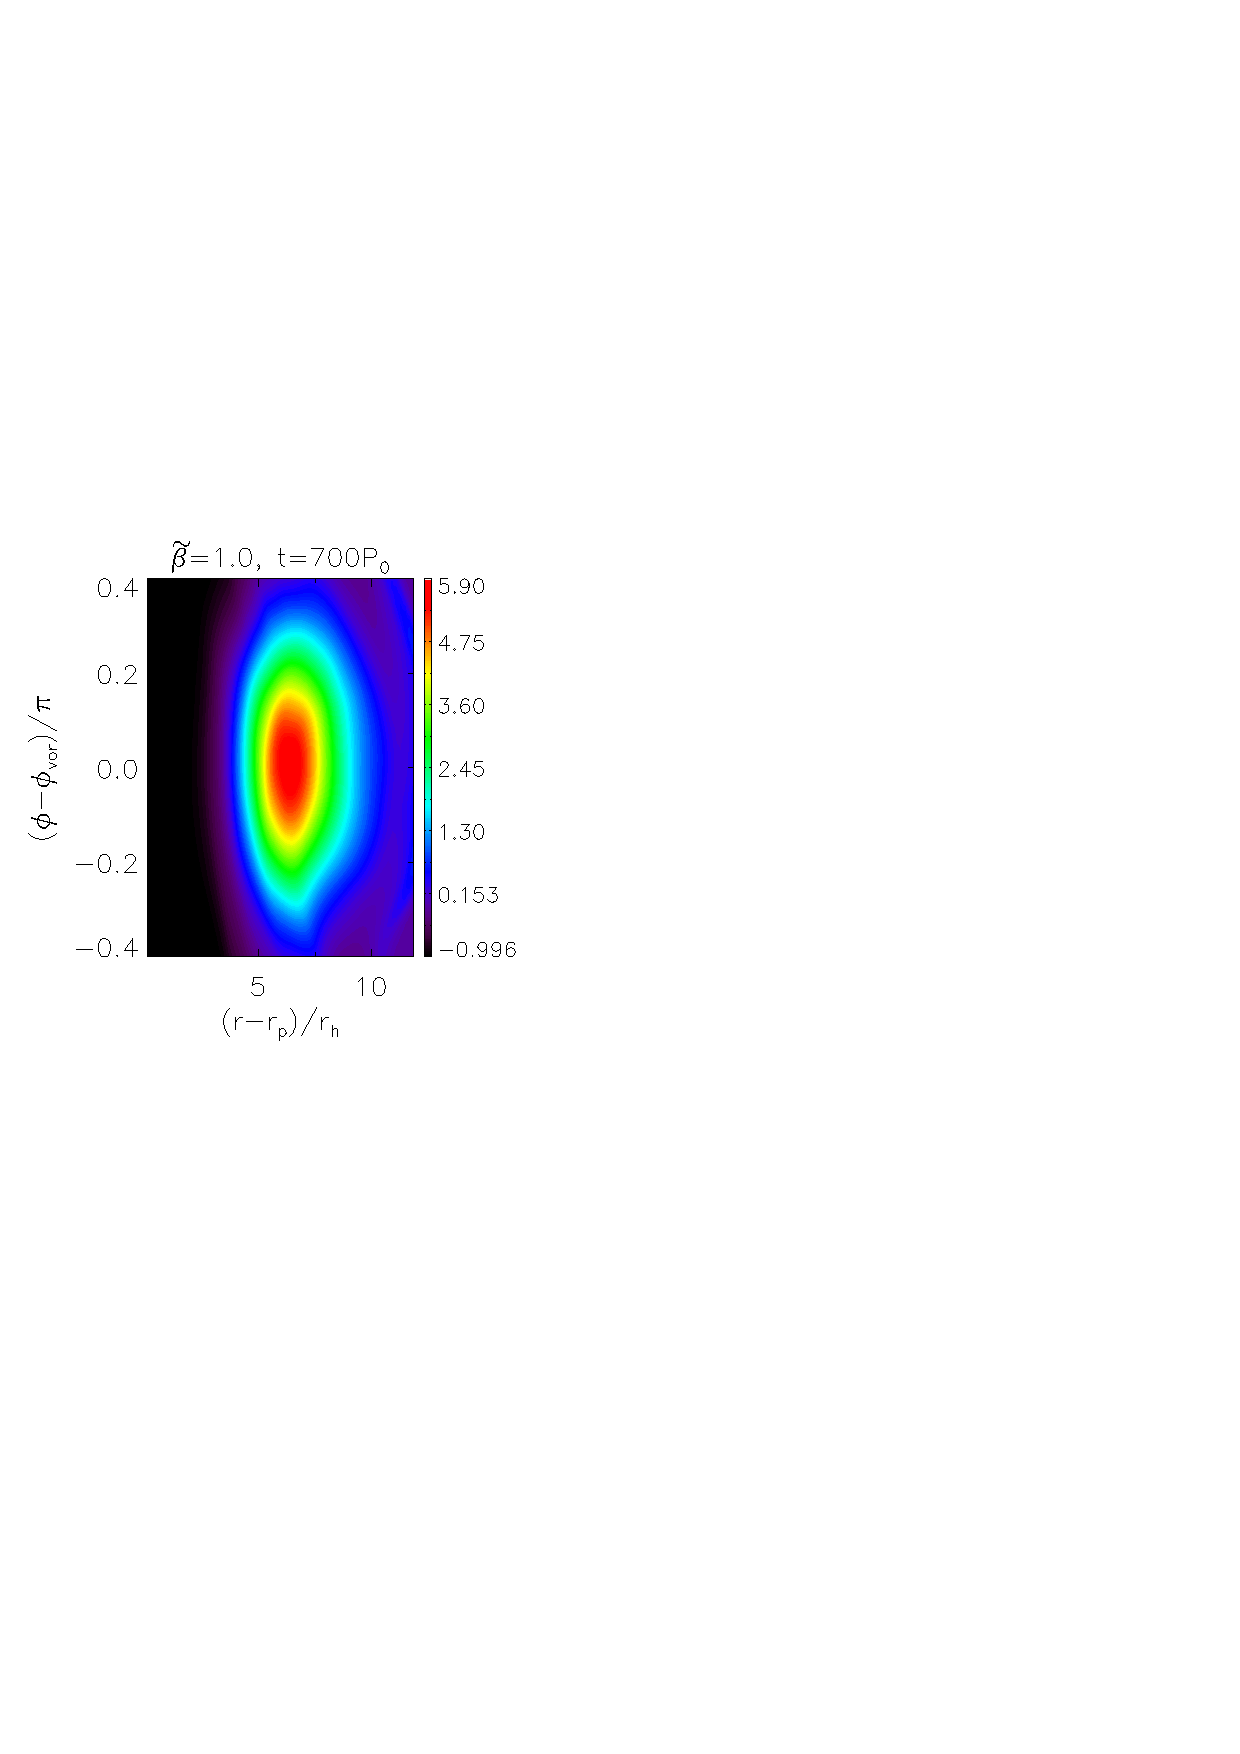
\includegraphics[width=0.3\linewidth]{figures/shock1}
  }
\hfill
  \subfigure{
    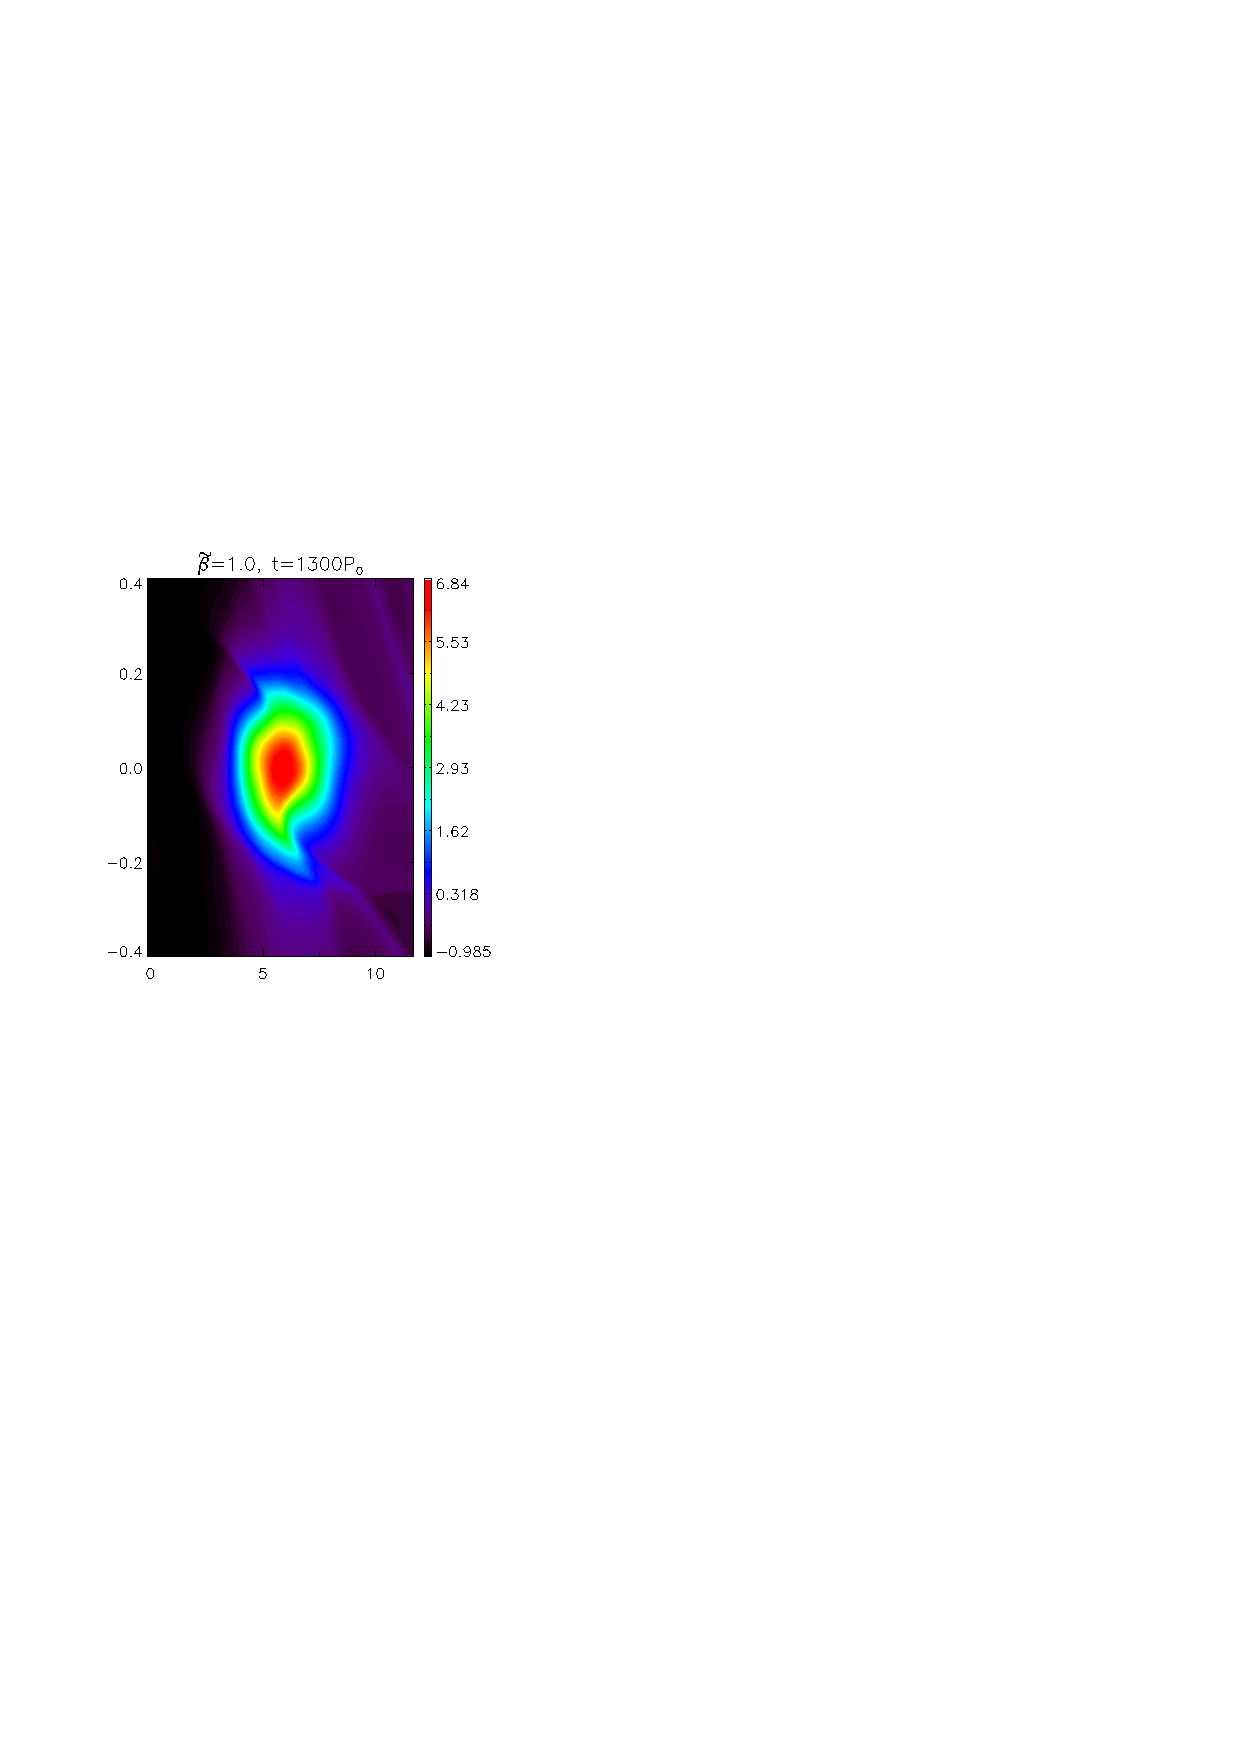
\includegraphics[width=0.3\linewidth]{figures/shock2}
  }
\hfill
  \subfigure{
    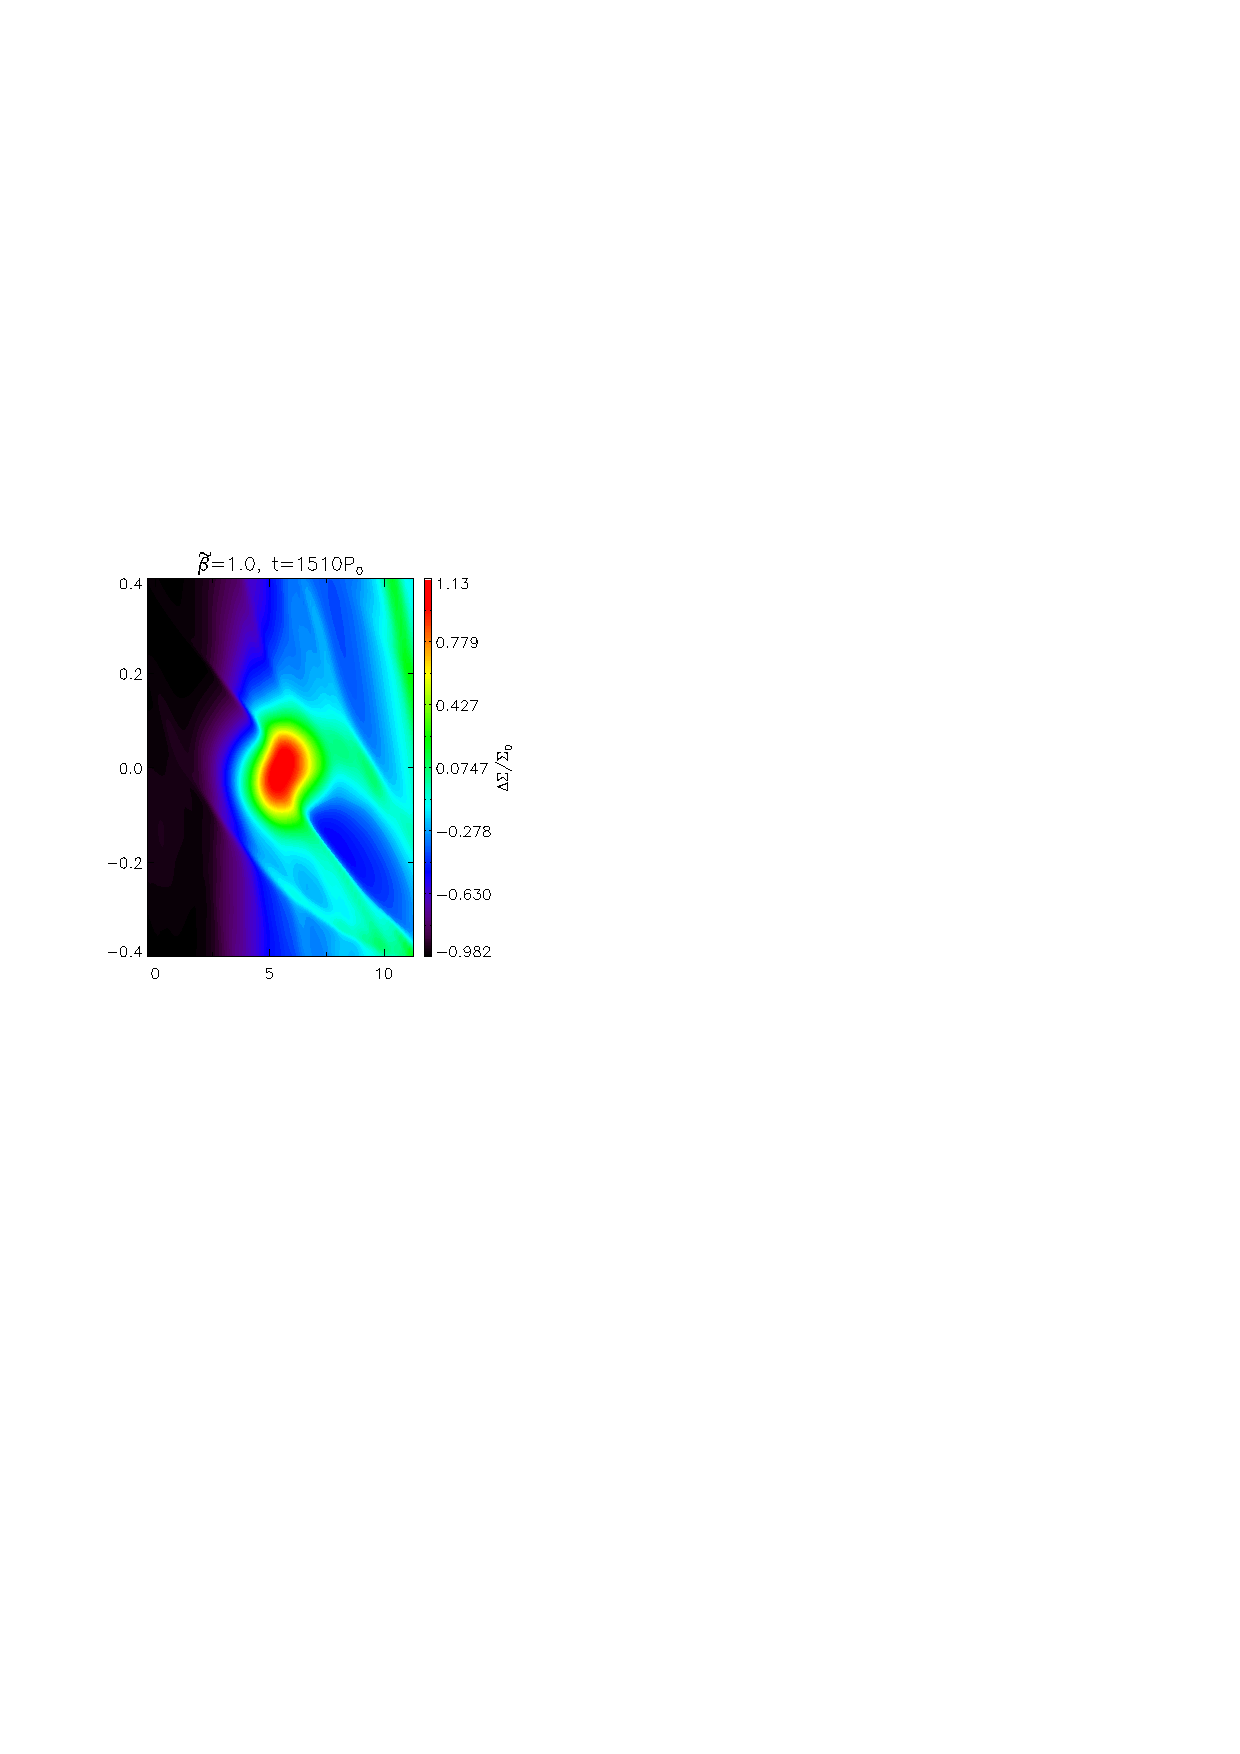
\includegraphics[width=0.3\linewidth]{figures/shock3}
  } \\[-0.98cm]
\subfigure{
    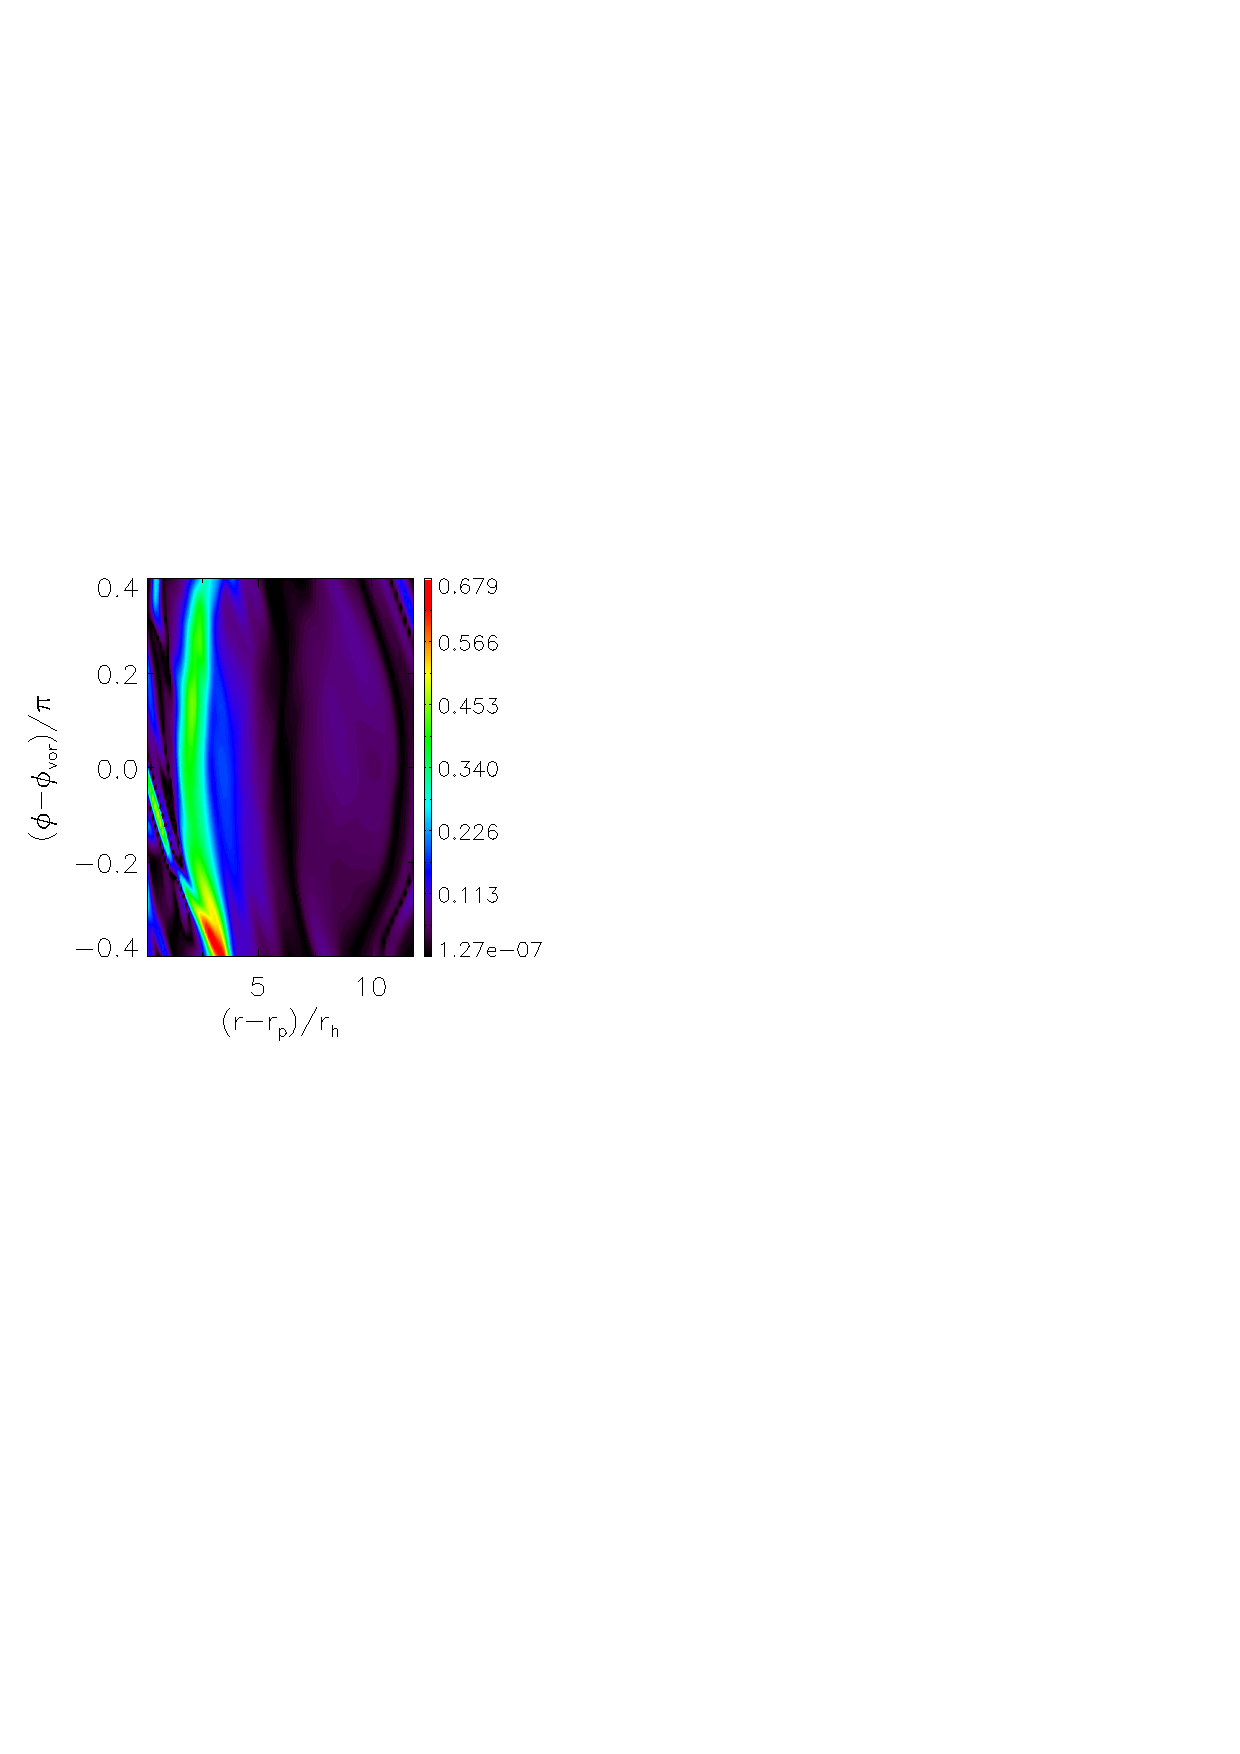
\includegraphics[width=0.3\linewidth]{figures/shock4}
  }
\hfill
  \subfigure{
    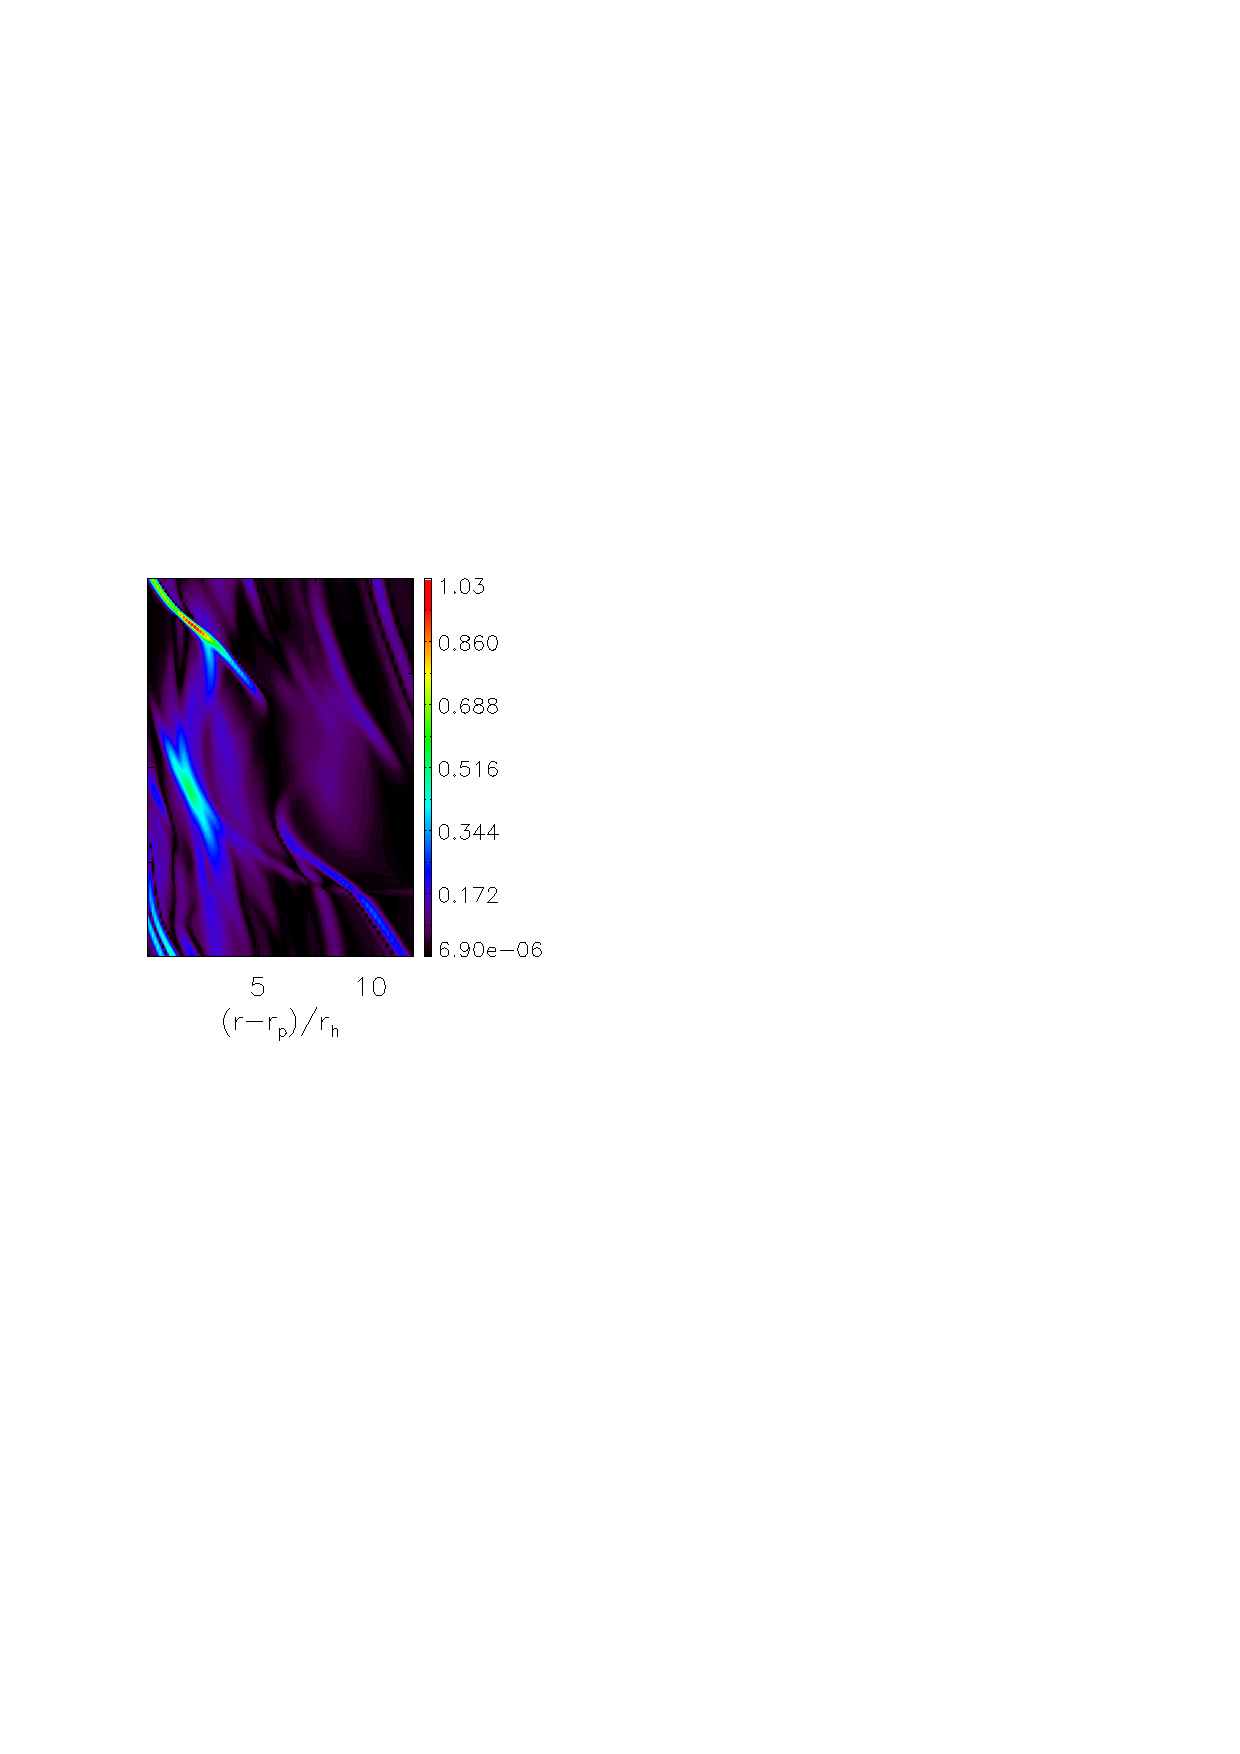
\includegraphics[width=0.3\linewidth]{figures/shock5}
  }
\hfill
  \subfigure{
    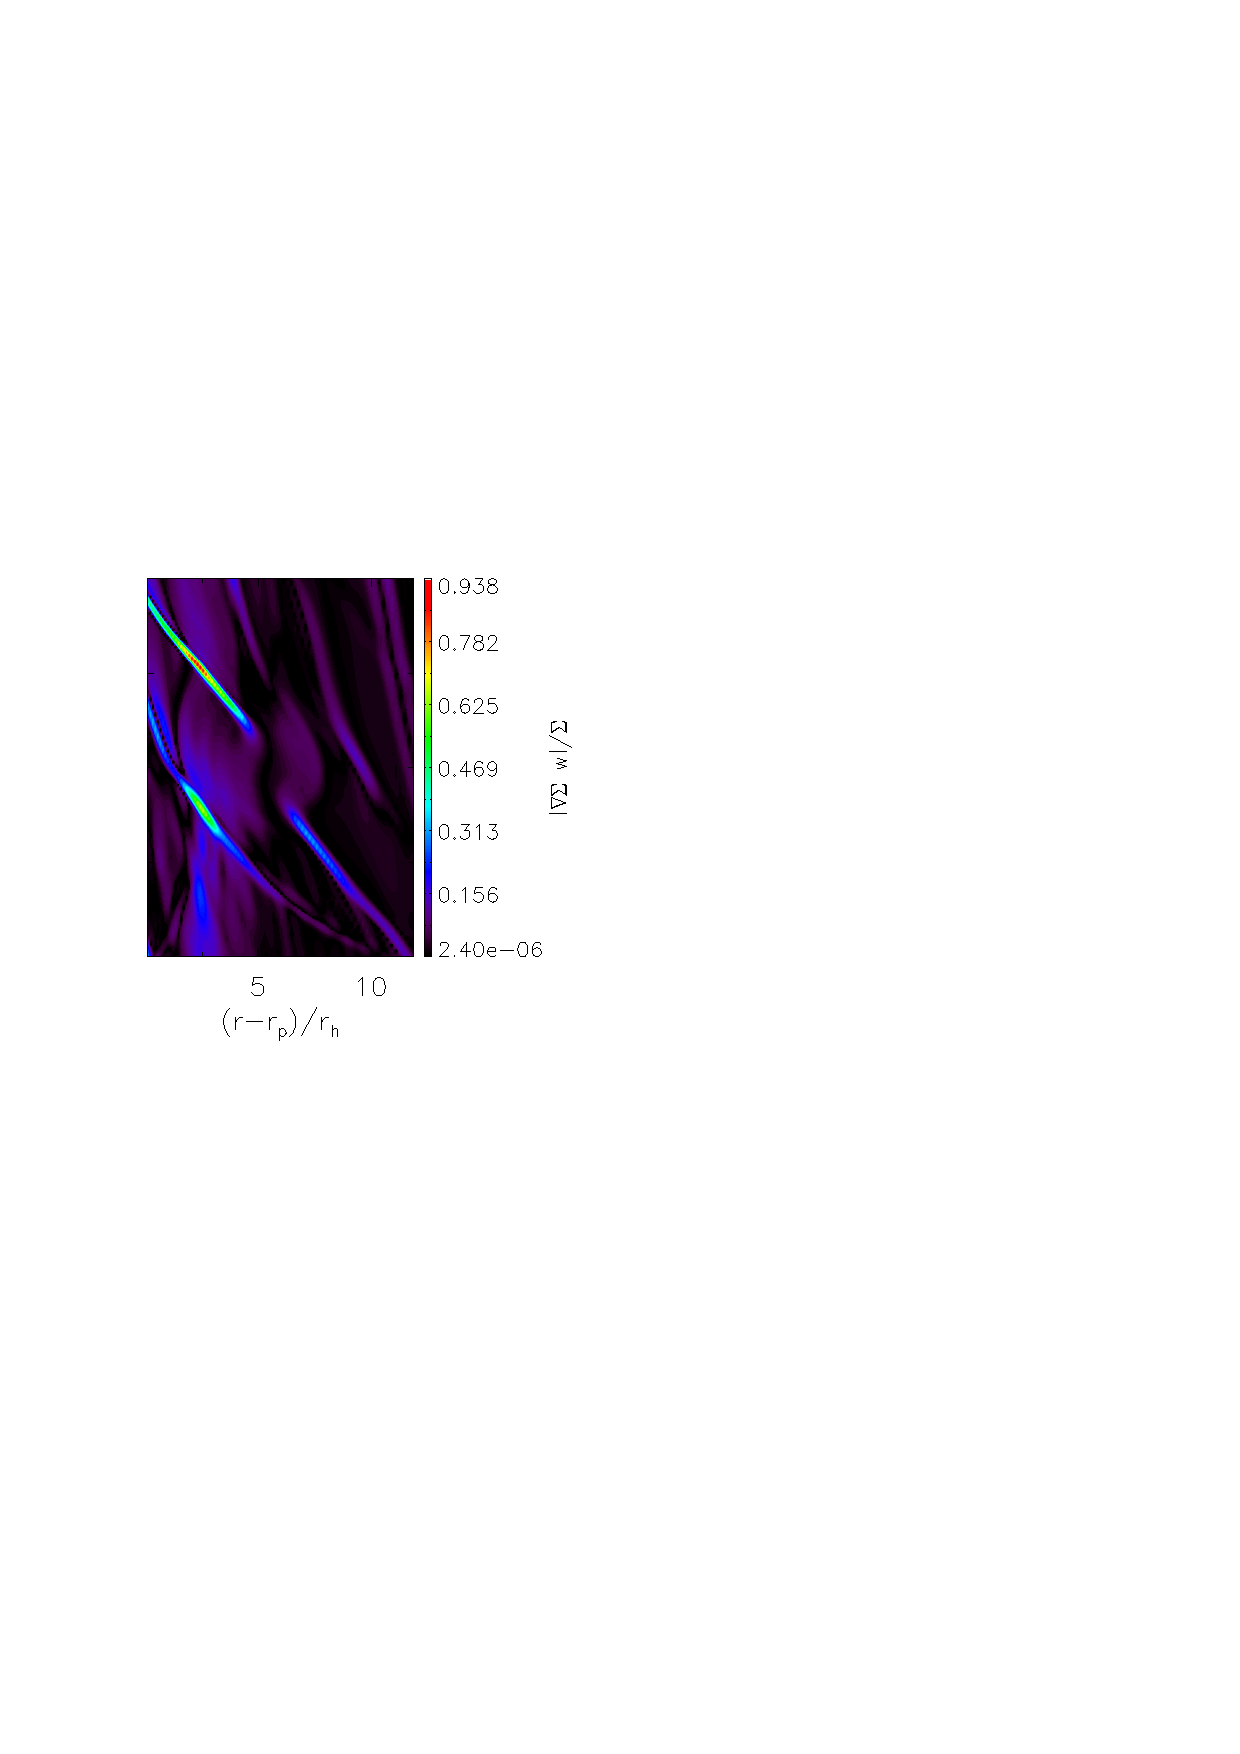
\includegraphics[width=0.3\linewidth]{figures/shock6}
  } 
  \caption{Relative density pertibation of vortices (top) and density gradient
 (bottom) for before (left), during (middle) and after dissipation (right).
 Large density gradients are characteristics of shocks and become prominant
 around vortex during dissipation} \label{shockplot}
\end{figure}

\begin{figure}
    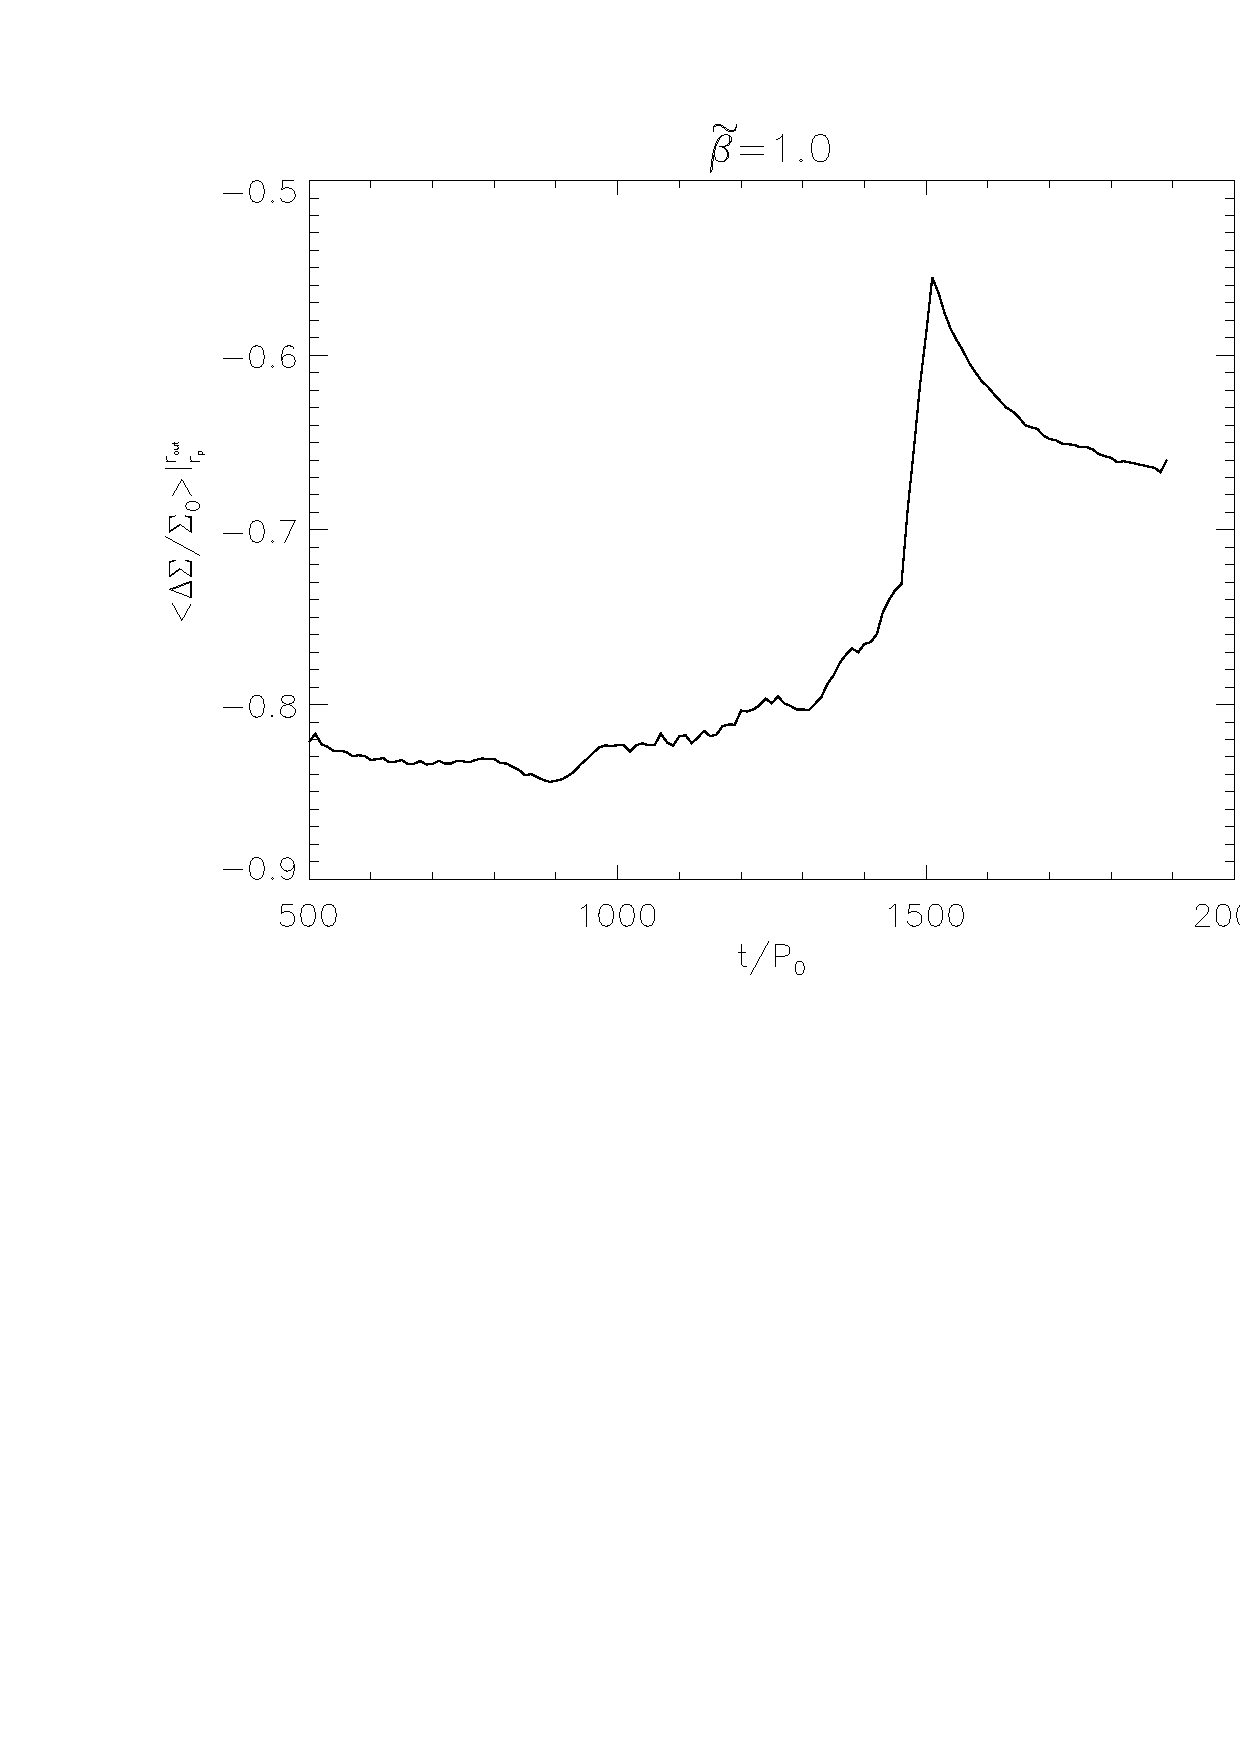
\includegraphics[width=\linewidth]{figures/gapdepth}
 \caption{Running average of relative density pertibation within the outer half
of gap} \label{gapdepth}
\end{figure}
\subsection{Vortex lifetimes as a function of cooling rate}

{\bf describe dependency on
cooling. Do we have enough data to have a `lifetime v.s. beta'
  plot? here we want to explain why vortex lives longer with longer
  cooling, but very long cooling results in shorter lifetimes. 
  Consider the following quantities as a function of cooling:
  initial strength of the single vortex; growth rate of single vortex
  strength from its formation to just before death; ampiltude of
  vortex just before death; disc temperature in the vortex region. 

  we expect the initial $m=1$ vortex (after merging) to be weaker with
  increasing cooling time because the instability is weaker. (see
  meheut et al 2013, mnras, 430, 1988 who show that the initial vortex
  amplitude after linear growth is correlated with the linear growth
  rate). 

  suppose the vortex shocks when it reaches a certain amplitude (which
  probably increases with longer cooling rate because it's more
  difficult to shock a hotter disc). as we
  increase the cooling time, the initial $m=1$ vortex is weaker, it
  also grows more slowly because gap-opening is opposed by a hotter
  disc. the above implies that it takes longer for the vortex reach
  the shock-inducing amplitude and dissipate.  

  but the above is not consistent with non-monotonic behaviour, which
  predicts the $\tilde{\beta}=10$ vortex to survive longest. this is
  because we expect the initial vortex to be weakest (check) which
  means it should take the longest to grow and shock. check
  whether there's anything special about this case. one possibility is
  that vortex growth during the quasi-steady state is actually faster
  because of the raised temperature (li et al 2000 show increased
  temperature favours RWI - possibiliy evidenced here by a stronger
  vortex before death than other cases) 

  perhaps have a case of $\tilde{\beta}=7.5$ as further evidence of
  non-monotonic behaviour
}

Fig. \ref{lifetimeplot} shows that increasing $\tilde{\beta}$
increases the lifetime of the vortex up to a critical 
value $\tilde{\beta}=5.0$ for which the vortex lasted beyond the
simulation time of $2000P_0$. This is consistent with vortex
dissipation when it induce shocks. Our `planet-off' simulations
indicate weaker vortices are formed initially with increased cooling
times. After merging, the growth of the single vortex, mediated by disc-planet
interaction, is expected to be slower with increased cooling time
because gap-opening becomes more difficult in a hotter
disc. Furthermore, the increased sound-speed suggest the vortex should
reach larger amplitudes in order to induce shocks. 
These expectations
imply that it takes longer for the vortex to induce shocks and
dissipate, and hence longer lifetimes with increasing
$\tilde{\beta}$. 

However, Fig. \ref{lifetimeplot} shows that increasing the cooling
time further to $\tilde{\beta}=10$ actually results in a
\emph{shorter} vortex lifetime. Notice for $\tilde{\beta}=10$ the vortex growth 
during the quasi-steady state is faster than for
$\tilde{\beta}=5$. This may be attributed to the higher temperature
reached in the former case ($h\simeq 0.08$). {\bf temperature for
  $\tilde{\beta}=5$?}, since \cite{li00} showed that the RWI grows
faster with increased disc temperature. At long cooling times, this
effect may dominate over the weaker gap-opening effect at higher $h$.   


Thus, unlike our `planet-off' simulations we find that there is
a cooling time $t_c$ which maximises the vortex lifetime. In the long term
 'planet-off' simulations we find that the vortices dissipate very gradually and visciously. {\bf to make
this comparison we need to discuss vortex lifetimes for planet-off
simulations as well} 
This
non-monotonic behaviour was also reported by \cite{fu14}, who
performed isothermal disc-planet simluations with different fixed
aspectratios.   
%Cooling rates with
%$\tilde\beta>5.0$ showed lifetimes that were well below the max
%lifetime. 
By analyzing the region
around the vortex {\bf define this region} we find the
$\tilde\beta=5.0$ case, with the longest vortex lifetime, has
$h\approx0.06$. This value of $h$ was also found to maximize vortex
lifetimes in the isothermal simulations of \cite{fu14}. 

%be the optimum lifetime for long-term simulations of
%isothermal disks with varying intial temperature profiles $h$. 

%Competing effects of gap stability with $t_{\mathrm{coo}l}$ result in
%the the non-montonic form of the lifetime. As the $\tilde\beta$
%increases so does the stability of the gap edge as seen in
%section~\ref{linear}, however as $\tilde\beta$ increases so does the
%$c_{\mathrm{iso}}$ which is known from theory to effect the growth of
%instability \citep{li00}. Thus increasing $\tilde\beta$ increases the
%sound speed $c_{\mathrm{iso}}$ and likewise the gap instability up to
%a certain point in which the effects of the more stable gap edge
%becomes a significant effect. 

%The correlation of growth rate and sound
%speed is non-negligible as in previous `planet-off' case as the disk
%now can reach values of $h\simeq0.08$ for very slow cooling and the
%importance of the effect can be imagined to accumulate over the now
%considerably longer timescale. These effects dictate when then the
%vortex reaches the critical value in which it shocks the system that
%subsequently causes disspation and hence the lifetime fo the vortex. 






